\documentclass[11pt,twocolumn]{article}
\usepackage[margin=0.8in]{geometry}                % See geometry.pdf to learn the layout options. There are lots.
\geometry{letterpaper}                   % ... or a4paper or a5paper or ... 
%\geometry{landscape}                % Activate for for rotated page geometry
%\usepackage[parfill]{parskip}    % Activate to begin paragraphs with an empty line rather than an indent
\usepackage{color}
\definecolor{myblue}{rgb}{0.0, 0.0, 0.85}
\usepackage[breaklinks=true, colorlinks=true, linkcolor=red, urlcolor=myblue, citecolor=black]{hyperref}
\urlstyle{rm}
\usepackage{amsmath}
\usepackage{mathptmx}
\usepackage{graphicx}
\usepackage{amssymb}
\usepackage{epstopdf}
\usepackage{sidecap}
\usepackage{authblk}
\usepackage{booktabs}
\usepackage[font=small,labelfont=bf]{caption}
\DeclareGraphicsRule{.tif}{png}{.png}{`convert #1 `dirname #1`/`basename #1 .tif`.png}
\usepackage{enumitem}
\setlist[itemize]{noitemsep}
\setlist[enumerate]{noitemsep}

\def\bfr{\bf\color{red}}
\def\geohub{{\tt geohub}}
\def\Count{count}
\def\ntracts{39}
\def\nprof{9}
\def\nvol{30}
\def\resp{respectively}
%\raggedbottom

\title{\bf
	Results of the 2021 Greater Hollywood Volunteer Homeless Count
	}
\author[1,2,3,$\dagger$]{Louis Abramson}
\author[4]{Brian Kohan}
\author[1,5]{Jackie Vorhauer}
\author[1,6]{Heather Carmichael}
\author[1,7]{Helen Eigenberg}
\author[1,8]{Stephen Fiechter}
\author[1]{David Gordon}
\author[9]{Courtney Kanagi}
\author[1,10]{Emily Uyeda Kantrim}
\author[9]{Guido Merkens}
\author[1,10]{Arnali Ray}
\author[5]{Elyse Schwartz}
\author[1,5]{Douglas Walker}
\author[1]{Kerry Morrison}
\affil[1]{\it \small Hollywood 4WRD Homelessness Coalition, 6255 Sunset Blvd, Ste 150, Los Angeles, CA 90028}
\affil[2]{\it Central Hollywood Neighborhood Council, PO Box 93907, Los Angeles, CA 90093}
\affil[3]{\it Carnegie Observatories, 813 Santa Barbara St, Pasadena, CA 91101}
\affil[4]{\it SELAH Neighborhood Homeless Coalition, \bf address}
\affil[5]{\it The Center at Blessed Sacrament, 6636 Selma Ave, Los Angeles, CA 90028}
\affil[6]{\it My Friend's Place, 5850 Hollywood Blvd, Los Angeles, CA 90028}
\affil[7]{\it Hang Out Do Good, \bf address}
\affil[8]{\it People Assisting The Homeless, 340 N Madison Ave, Los Angeles, CA 90004}
\affil[9]{\it The Hollywood Partnership, 6562 Hollywood Blvd, Los Angeles, CA 90028}
\affil[10]{\it Mid City West Community Council, 644 N Fuller Ave, PMB 7059, Los Angeles, CA 90036}
\affil[$\dagger$]{Corresponding author; \href{mailto:labramson.chnc@gmail.com}{labramson.chnc@gmail.com}}

\date{\vspace{-1em}Draft: \today}                                           % Activate to display a given date or no date

\begin{document}
\maketitle

\begin{abstract}

Data from February 25, 2021 censuses of Hollywood and East Hollywood shows that 
unsheltered homelessness has fallen in those communities by $11\%\pm9\%$ and 
$15\%\pm12\%$, \resp, compared to the 2020 LAHSA Point-In-Time (PIT) count (90\% CI). 
A 30\% drop in individuals seen on the street drives this change, reducing the number of identified 
persons and dwellings in about a third of census tracts. Unsheltered living is thus likely to have 
declined quantitatively even if the average occupancy of, e.g., tents is updated. Simultaneously, 
however, 13\% of tracts saw at least a doubling in street dwellings. This trend may contribute to 
qualitative perceptions that the state of homelessness has worsened over the past year, which---given 
COVID-related reductions in health, hygiene, and social support services---are also likely to be accurate.
Coordinated Entry System data will reveal whether homelessness has declined in toto or if 
government initiatives reduced only the portion of people living unsheltered in Greater Hollywood.

\end{abstract}

\section{Context}
\label{sec:intro}

The Los Angeles Homelessness Services Authority (LAHSA) conducts an annual Point In Time (PIT) 
census of the unhoused population of Los Angeles County. These data inform programmatic
funding levels, educate residents, undergird legislative efforts, and shape the day-to-day practices of 
professional and volunteer service providers. 

As the official assessment of the scope of one of the most pressing humanitarian issues of our time, 
the LAHSA Count is invaluable. However, due to disruptions from COVID-19, the unsheltered portion 
of the 2021 PIT count was cancelled. Since 70\% of the unhoused residents of the City of LA (``LA'')
were unsheltered as of 2020, absent additional efforts, this cancellation would substantially erode 
our understanding of the state of homelessness following an unprecedented year of economic disruptions 
and governmental interventions---both of which may have significantly affected the number of unhoused 
Angelenos.

Greater Hollywood is an epicenter of the homelessness crisis. According to the 2020 Count, the 
Hollywood and East Hollywood Communities were home to 2203 unhoused residents, 1714 of whom 
(78\%) were unsheltered. This figure corresponds to roughly 
\href{https://www.lahsa.org/data?id=45-2020-homeless-count-by-community-city}
{5\% of LA's homeless population} in an area with \href{https://geomap.ffiec.gov/FFIECGeocMap/GeocodeMap1.aspx}{3.5\% of its total population}. In some places, 1-in-25 Hollywood residents are 
unhoused compared to 1-in-100 citywide.

\begin{figure*}
	\centering
	\includegraphics[width=0.9\linewidth]{countMap}
	\caption{The 2021 volunteer \Count\ covered Greater Hollywood, comprising the 
			officially recognized LAHSA Hollywood and East Hollywood Continua
			of Care. The former stretches from Laurel Canyon Blvd to Western Ave,
			the latter from Western to Hoover Ave. Hollywood is bounded to the north
			and south respectively by Franklin	and Melrose Aves, with East Hollywood
			bounded by Hollywood Blvd and Beverly Ave. Hollywood comprises
			21 census tracts; East Hollywood 18.}
	\label{fig:map}	
\end{figure*}

While the above statistics are tragic, Hollywood is also home to large and increasingly formalized
coalitions of service providers, business leaders, residents, and governmental entities dedicated to 
humanely housing everyone in their neighborhood. Given the capacity of the above organizations and 
the importance of the annual PIT count in educating residents, funders, and legislators, Hollywood 
proceeded as a collective to conduct an unsponsored grassroots PIT \Count\ in on Thursday, 
February 25, 2021.

This document details the methodology and findings of that \Count. 
Section \ref{sec:procedure} describes the volunteer training, data acquisition, 
and analysis protocols. Section \ref{sec:results} presents estimates of the unsheltered 
populations in Hollywood and East Hollywood, contextualizes those in terms of the 2020 
LAHSA PIT results and those communities' total populations, and presents cross-checks. 
Section \ref{sec:discussion} provides interpretation, highlights areas for further study, and 
reveals where quantitive findings may drive qualitative impressions as to the ``felt'' state of 
the crisis. Section \ref{sec:summary} summarizes. The Appendix provides additional information, 
including tract-level raw tallies and population inferences. All data are available at {\bfr website}.

\section{Methodology}
\label{sec:procedure}
%
%The \Count\ took place on 25 February 2021 circa at 7.00 PM. This timing corresponds to one month 
%after and four hours before the official event would have occurred. Beyond those choices, our program 
%adhered as closely as possible to the official LAHSA 2020 PIT data collection and analysis protocols. 
%
%The \Count\ was launched from The Center at Blessed Sacrament (``The Center''), a major service 
%provider in Hollywood, at 6636 Selma Ave. All volunteer teams reported and returned to this 
%location as they would to a LAHSA community hub in past years, but, as COVID precautions, 
%training was performed remotely in the week preceding the count and volunteers never left their 
%vehicles.

\subsection{Data Acquisition}
\label{sec:acquisition}

The \Count\ was based out of The Center at Blessed Sacrament (``The Center''), a major service 
provider in Hollywood. All volunteers reported and returned to this location as they would a LAHSA 
community hub in the past. Unlike previous PIT counts, however, training was performed offsite, 
volunteers never left their vehicles, and all surveying occurred before 10:00 PM.

The \Count\ covered the \ntracts\ US Census tracts constituting the LAHSA-defined 
\href{https://www.lahsa.org/data?id=45-2020-homeless-count-by-community-city}{Hollywood 
and East Hollywood Communities} (21 and 18 tracts, \resp). It did not recognize census 
tract ``splits''---e.g., ``1905.10a''---which modified of the definition of Hollywood to include 
all of tract 1905.10 and East Hollywood to include all of tract 1913.01. Since 2016, tract 1905.10b 
has never hosted more than 7 unsheltered people and 1913.01a never more than 15. As such,
these modifications do not significantly affect community-level results.
%Sections \ref{sec:results} and \ref{sec:discussion} discuss community-level results with 
%tract-level tallies provided in the Appendix. Results for Greater Hollywood are not directly comparable 
%to any official service geography but are available upon request. 
Figure \ref{fig:map} shows the \Count\ footprint.

All tracts were vetted by outreach professionals from The Center prior to assignment. Tracts 
deemed especially challenging---e.g., due to their proximity to freeway onramps/peripheries---were 
reserved for professional counting teams. Vetting produced \nprof\ such tracts, which were surveyed 
by personnel from The Center and Covenant House circa 3:00 PM on 25 Feb. The remaining \nvol\ 
tracts were divided among the volunteer vehicle-based teams and surveyed beginning at 7:00 PM. 

With 
the exception of one tract in East Hollywood, teams were restricted to one or the other community, 
making the community-level results nearly independent. Cross-comparisons therefore serve as data 
quality indicators (Section \ref{sec:crossChecks}). Table \ref{tbl:tractStats} records which tracts were 
surveyed by which kind of team. 

Thirty-two volunteer teams participated in the \Count, which was limited to existing ``pods'' of two 
to three people to minimize the possibility of COVID transmission. 
%Singlet volunteers were admitted 
%but remained on-site to assist with traffic control and material distribution. 
All participants wore 
personal protective equipment and maintained social distancing when appropriate.

Counting followed 2020 LAHSA PIT protocols to the greatest extent possible. Each volunteer team 
comprised at least a driver and a counter and was assigned two tracts. Three-person teams 
included a navigator, as well. If present, the navigator directed the driver while the counter tallied 
individuals/dwellings. In two-person teams, the counter doubled as the navigator. Training 
emphasized techniques aimed at reducing counters' cognitive loads to minimize errors (e.g., 
covering interior streets in a serpentine pattern before circling the tract border). Teams were 
instructed to count both sides of interior streets but only interior sides of border streets 
as described in the official 2020 PIT training materials.

All teams were deployed by roughly 7:30 PM and returned by 9:55 PM.

Upon arriving at The Center, organizers provided each team a clipboard containing:
\begin{itemize}
	\item two tract maps;
	\item two tally sheets;
	\item one 1-page training summary with a contact number for field issues.
\end{itemize}

The tally sheets were the data acquisition tool. These contained separate columns for each of the 
nine categories of unhoused individuals/dwellings recognized in the 2020 LAHSA PIT count: 
\begin{enumerate}
	\item adults (ages $\geq$25);
	\item transition age youths (``TAY,'' 18--24);
	\item unaccompanied minors;
	\item families (at least one adult with at least one minor); 
	\item cars;
	\item vans;
	\item RVs;
	\item tents;
	\item makeshift structures.
\end{enumerate}
Dwellings---(5)--(9)---are treated specially in the analysis and hereafter 
may be referred to by the acronym ``CVRTM.'' Adults+TAY may also be combined into 
``Persons'' (P). No families or unaccompanied minors were identified.\footnote{
One potential unaccompanied minor was reported in tract 1912.01 but could not be confirmed by outreach
personnel dispatched to that location. One potential family was also reported dwelling in a van in
tract 1899.05 that could also not be confirmed. The upper limits for these categories (3 each at 95\%
confidence) capture this uncertainty, but their raw counts are set to zero.} See Appendix for examples
of the above documents.

Upon returning, counters verbally read their results to organizers who entered them into a google 
form. The organizer read back the results for confirmation before submitting the form and recovering the
hand-written tallies from the volunteers. 
%Volunteer email addresses were also retained for follow-up. 

Once all materials were collected, organizers cross-checked the electronic records---a
google sheet generated by the google form responses---with the paper tally sheets and 
identified any uncounted areas. None were found that required follow-up. Disagreements 
between electronic and paper references were corrected to the paper tally. 
%All data are available at {\bfr website}.

Given turnout, every volunteer tract was counted by at least two teams. Four tracts were counted
in triplicate. Beyond increasing the accuracy of the count, repeat measurements enhance understanding of 
errors (Sections \ref{sec:dupes}) and provide robustness (one tally was uninterpretable, leaving only the 
result from the second assigned team).

All told, the data comprise 37 pair-wise volunteer measurements,
%---29 duplicates + 
%4 triplicates (=8 additional pairs)---
one unique volunteer measurement, and nine unique 
professional assessments. The latter account for $\sim$20\% of tracts in both communities and roughly 
43\% of the individuals and dwellings identified. Year-on-year trends are consistent between
volunteer- and professional-counted tracts (Section \ref{sec:crossChecks}). 
%The largest increase was observed by volunteers, the largest
%decrease by professionals.%; both tracts are located in E.~Hollywood.

\begin{table}[t!]
\caption{Tract-level Unsheltered Population Summary}
\resizebox{\linewidth}{!}{%
\begin{tabular}{cccccc}
\toprule
Tract & Community & Counter$^{\rm a}$ & Passes$^{\rm b}$ & Median Est. & 90\% CI \\ 
 & & & & [people] & [people] \\ \cmidrule{1-6}
1898.00 & Hollywood & Vol & 3 & 6 & 0--15 \\
1899.02 & Hollywood & Vol & 3 & 18 & 12--24 \\
1899.03 & Hollywood & Vol & 2 & 0 & 0--12 \\
1899.04 & Hollywood & Vol & 2 & 18 & 11--25 \\
1899.05 & Hollywood & Vol & 2 & 19 & 9--30 \\
1901.00 & Hollywood & Vol & 2 & 88 & 75--102 \\
1902.01 & Hollywood & Vol & 2 & 21 & 13--29 \\
1902.02 & Hollywood & Vol & 2 & 30 & 20--40 \\
1903.01 & Hollywood & Pro & 1 & 74 & 54--96 \\
1905.10 & Hollywood & Pro & 1 & 34 & 22--46 \\
1905.20 & E.~Hollywood & Vol & 2 & 12 & 6--18 \\
1907.00 & Hollywood & Vol & 2 & 110 & 93--127 \\
1908.01 & Hollywood & Vol & 2 & 63 & 50--76 \\
1908.02 & Hollywood & Pro & 1 & 71 & 54--90 \\
1909.01 & Hollywood & Pro & 1 & 55 & 39--71 \\
1909.02 & Hollywood & Vol & 3 & 6 & 0--17 \\
1910.00 & Hollywood & Pro & 1 & 169 & 140--201 \\
1911.10 & E.~Hollywood & Vol & 2 & 9 & 2--15 \\
1911.20 & E.~Hollywood & Pro & 1 & 66 & 48--85 \\
1912.01 & E.~Hollywood & Vol & 2 & 55 & 44--68 \\
1912.03 & E.~Hollywood & Vol & 2 & 26 & 14--38 \\
1912.04 & E.~Hollywood & Vol & 2 & 6 & 0--16 \\
1913.01 & E.~Hollywood & Vol & 2 & 31 & 22--42 \\
1913.02 & E.~Hollywood & Vol & 2 & 23 & 15--30 \\
1914.10 & E.~Hollywood & Vol & 2 & 20 & 13--28 \\
1914.20 & E.~Hollywood & Vol & 2 & 24 & 16--32 \\
1915.00 & E.~Hollywood & Vol & 2 & 29 & 21--38 \\
1916.10 & E.~Hollywood & Pro & 1 & 48 & 31--68 \\
1916.20 & E.~Hollywood & Pro & 1 & 17 & 6--30 \\
1917.10 & Hollywood & Vol & 2 & 21 & 14--29 \\
1917.20 & Hollywood & Vol & 3 & 21 & 12--31 \\
1918.10 & Hollywood & Vol & 2 & 24 & 14--34 \\
1918.20 & Hollywood & Vol & 2 & 16 & 10--23 \\
1919.01 & Hollywood & Vol & 2 & 60 & 49--72 \\
1925.10 & E.~Hollywood & Vol & 2 & 12 & 4--21 \\
1925.20 & E.~Hollywood & Vol & 1 & 14 & 1--28 \\
1926.10 & E.~Hollywood & Vol & 2 & 7 & 1--14 \\
1926.20 & E.~Hollywood & Vol & 2 & 18 & 9--26 \\
1927.00 & E.~Hollywood & Pro & 1 & 129 & 96--167\\
\cmidrule{1-6}
{\bf All} & & & {\bf 72}$^{\rm c}$ & {\bf 1494} & {\bf 1342--1657}
\\ \bottomrule
\end{tabular}
}
\caption*{$^{\rm a}$Volunteer vs.~professional surveyor; $^{\rm b}$independent 
		tract counts; $^{\rm c}$reflects one tally rejected during quality control.}
\label{tbl:tractStats}
\end{table}

\subsubsection{Volunteer Training}
\label{sec:training}

Teams underwent mandatory, $\sim$30 minute Zoom-based training sessions before arriving 
for the \Count. Each participant was also required to watch the official 2020 LAHSA PIT training 
video.% and sign participation waivers.

The training covered the motivation for the \Count, an overview of the survey geography, team roles, 
and examples of unhoused dwellings. Except in the case of people standing next to tents---as described 
in the 2020 LAHSA video---volunteers were instructed to count CVRTM and individuals separately 
and not to try to estimate how many people might live in or be associated with a specific dwelling. 
This ensured that results could be analyzed as a function of the CVRTM weights, which may change 
with future information.% (see Section \ref{sec:analysis}).

Volunteers were primed only with min/max estimates of tract-level individual+dwelling counts 
(``0--120'') and the likelihood of encountering unaccompanied minors or families (``very unlikely'')
or TAY (``some tracts especially in Hollywood''). These statements were informed by the 2020 LAHSA PIT 
results. No other prior was established. The training presentation is available 
at: \url{https://drive.google.com/file/d/1xFrtU26yjPuiUv9KHZ3Uj2_sAoT1ClGo/view?usp=sharing}.

\subsection{Data Analysis}
\label{sec:analysis}

The data form a $9\times73$ array containing the tract-level tallies for each unhoused 
individual/dwelling class. Analysis involves averaging duplicate tract counts,
associating the latter with the Hollywood or East Hollywood communities, and 
weighting CVRTM by their mean occupancies. The final data product reflects 10,000 realizations 
of the total population inference incorporating random perturbations of the counts and weights 
according to their uncertainties (see below). It forms a $9\times10000\times39$ array that 
may be split and summed to provide aggregate, tract, or category-level population estimates and 
uncertainties.

Our baseline result incorporates the \href{https://www.lahsa.org/documents?id=4686-2020-greater-los-angeles-city-community-homelessness-report-service-planning-area-4.pdf}{2020 SPA-4/CD13 CVRTM weights}
underpinning the 2020 LAHSA \href{https://www.lahsa.org/documents?id=4686-2020-greater-los-angeles-city-community-homelessness-report-service-planning-area-4.pdf}
{Community Summaries}. We recognize that these weights may have changed since they were last
estimated. We cannot reassess all of them and encourage robust efforts to do so. However, at 
least one survey of tent-dwellers in Hollywood suggests the tent weight, $T$, has not changed 
significantly. We analyze the impact of adopting three other reasonable CVRTM choices in 
Section \ref{sec:comp} (Table \ref{tbl:weights}), but they do not significantly affect our findings.
%COVID-related activities such as tent  distribution efforts may have changed

%While an estimate of the underlying population, uncertainties in each visual count and weight 
%must be accounted for to understand how confident one can be that that estimate corresponds to
%the truth. We accomplish this by using Monte Carlo integration to construct the full probability
%distribution functions (PDFs) for the number of unsheltered people of each class in each tract.

% {\it These results will
%correspond to the most likely values for the respective quantities in any geography.} However,
%three uncertainties---one small and two large---complicate the interpretation of those sums. 
%We discuss these in Section \ref{sec:discussion}, but account for them as best we can using 
%Monte Carlo techniques to construct the full underlying probability distribution functions (PDFs) 
%for each class in each tract.
%
%All results discussed below derive from 10,000 Monte Carlo realizations of Item (5), above.
%

\subsubsection{Monte Carlo Population Inferences}
\label{sec:mc}

We wish to infer the true unsheltered population in Hollywood and East Hollywood as of 25 February. 
We do so by constructing probability density functions (PDFs) describing the likelihood of encountering 
a given number of unsheltered people in those communities as constrained by our PIT \Count. 
To accomplish this, we model three known uncertainties: (1) errors in the visual tallies, (2) deviations 
of the CVRTM weights from their quoted means, and (3) the intrinsic background rate of persons/dwellings
in areas in which none were actually sighted. Items (1) and (3) reflect how our PIT tally might change
if performed at a different time or by different teams. Item (2) reflects how the mean 
occupancy of CVRTM in our survey area might differ from that in the geography in which the weights 
were defined.

We model (1) and (2) as independent random draws from Gaussian distributions with standard 
deviations of $\sqrt{n}$ and $\sigma$, \resp, where $n$ is the raw PIT tally and $\sigma$ is the 
standard error on the respective CVRTM weight, $w$, quoted by LAHSA. The $i$-th 
estimate of the true number, $N$, of people belonging to the $j$-th unsheltered class in any tract is then:
\begin{multline}\label{eq:monte}
	N_{i,j} = \left[n_{j} + \mathcal{G}_{i}(0,\sqrt{n_{j}})\right]\times\max[\mathcal{G}_{i}(w_{j}, \sigma_{j}),1],
\end{multline}
where $\mathcal{G}(\mu,\Sigma)$ is a Gaussian random number with mean $\mu$ and standard deviation 
$\Sigma$. If more than one team counted a given tract, $n$ is replaced by the average of their tallies 
and the attendant counting error is divided by the square root of the number of teams. If no members
of the $j$-th unsheltered category were observed, $\sqrt{n_{j}}$ is replaced in the first term 
by that category's estimated background rate, $\sigma_{j}^{\rm bkg}$, discussed in the next section.% \ref{sec:nulls}).

The final output PDFs are based on 10,000 realizations of Equation \ref{eq:monte}. Weights for 
adults and TAY are fixed to unity, such that 
$(w,\sigma)\equiv(1,0)$ for all trials and uncertainties reflect only counting errors. One potential 
family and one potential unaccompanied minor were reported, but not confirmed. We therefore
set those entires to zero and infer only upper limits.

We place a floor on the CVRTM mean occupancies at 1 person per dwelling; i.e., we assume that the 
{\it mean} person does not own more than one dwelling. This is not to say no one may own more than 
one, just that such a statement is never representative. This choice induces a mild asymmetry in our 
global PDFs but does not significantly affect inferences.
%letting the mean occupancies reach 0 moves the baseline result down by 40 ppl over all of grtr Hwood.
%it's 0.4 sigma or in the IQR.

\begin{figure}[t]
\centering
	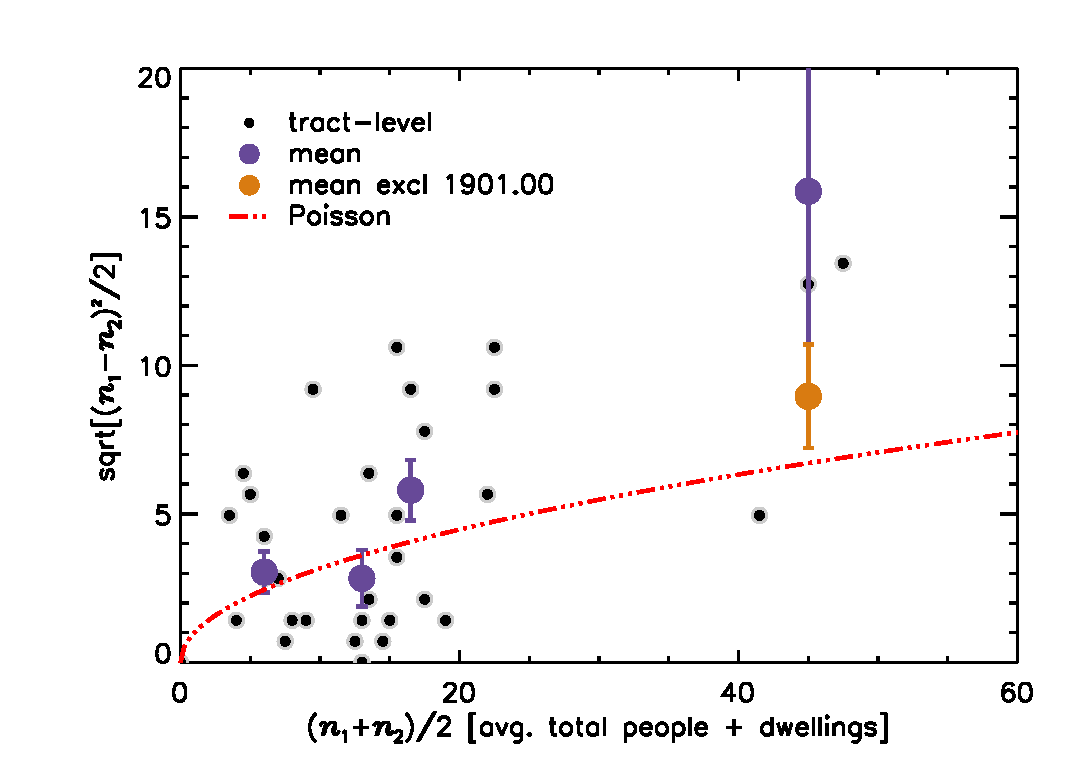
\includegraphics[width=\linewidth, trim = 1cm 0cm 0cm 0cm]{intDupeChar}\\
	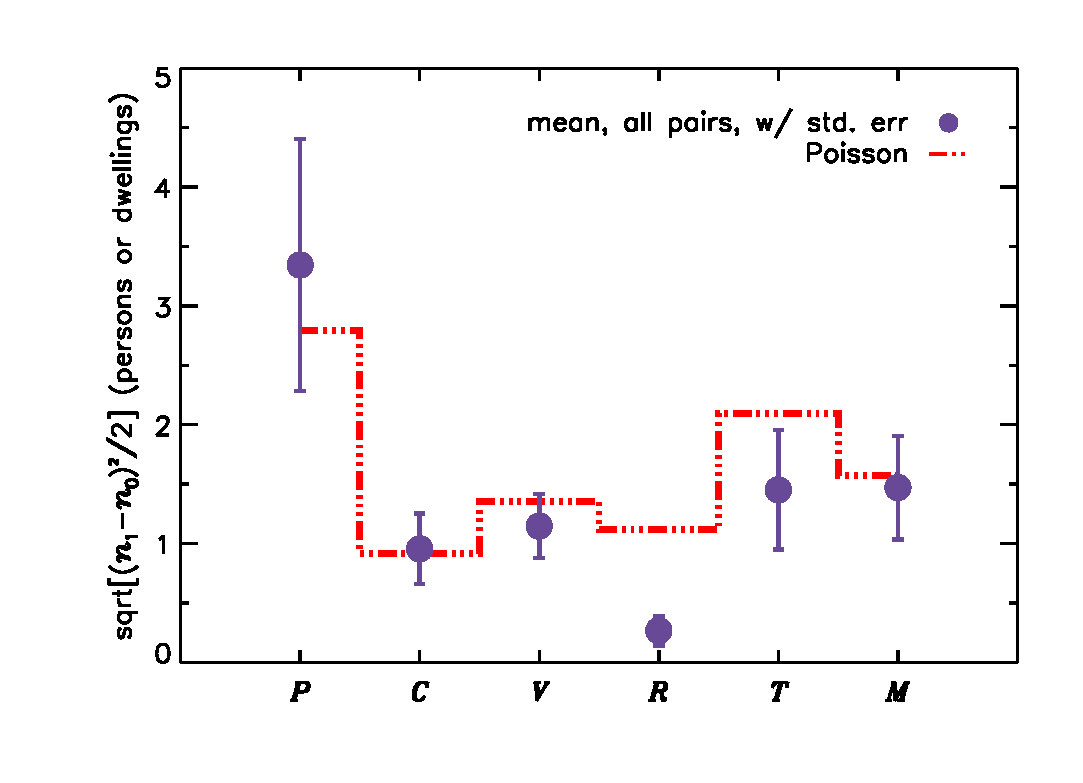
\includegraphics[width=\linewidth, trim = 1cm 0.5cm 0cm 0cm]{catDupeChar}
\caption{Duplicate tract (top) and category (bottom) count comparisons. Orange 
		points at top exclude tract 1901.00, which is a significant outlier.}
\label{fig:dupeChar}
\end{figure}
\subsubsection{Null Entries and Background Rates}
\label{sec:nulls}

Often, no persons or dwellings of a specific category are observed in a given census tract. Due to shot 
noise, however, such data are consistent with non-zero values for the true population. The Monte Carlo 
PDF reconstruction allows all such entries to fluctuate based on an assumed background rate,
$\sigma_{j}^{\rm bkg}$. 

\begin{table*}[t]
\centering
\caption{Greater Hollywood 2021 PIT Unsheltered Data and Population Estimates}
%\resizebox{\linewidth}{!}{%
\begin{tabular}{lccccc}
\toprule
 & $w_{C}$ & $w_{V}$ & $w_{R}$ & $w_{T}$ & $w_{M}$ \\ \cmidrule{1-6}
{\bf SPA4/CD13} & $1.51\pm0.25$ & $1.77\pm0.42$ & $1.42\pm0.28$ & $1.48\pm0.11$ & $1.68\pm0.31$ \\
2021 $T$ & -- & -- & -- & $1.39\pm0.14$ & --\\
2021 $T$ w/ unocc & -- & -- & --& $1.51\pm0.24$ & --\\
%2021 $T$ & $1.51\pm0.25$ & $1.77\pm0.42$ & $1.42\pm0.28$ & $1.39\pm0.14$ & $1.68\pm0.31$\\
%2021 $T$ w/ modeled unocc & $1.51\pm0.25$ & $1.77\pm0.42$ & $1.42\pm0.28$ & $1.51\pm0.24$ & $1.68\pm0.31$\\
SPA4 & $1.38\pm0.11$ & $1.68\pm0.22$ & $1.32\pm0.15$ & $1.45\pm0.06$ & $1.64\pm0.16$\\
\bottomrule
\end{tabular}
%}
\caption*{CVRTM weights tested. Dashes denote identical values to the entry above. Bold denotes 
baseline scenario incorporating the 
\href{https://www.lahsa.org/documents?id=4635-usc-2018-2020-multipliers-and-estimates-overview}
{2020 SPA4/CD13 CVRTM weights} underpinning the latest official Hollywood and East Hollywood 
\href{https://www.lahsa.org/documents?id=4686-2020-greater-los-angeles-city-community-homelessness-report-service-planning-area-4.pdf}{Community Summaries}.}
\label{tbl:weights}
\end{table*}

Ideally, that rate would be based on category variations in similar tracts defined by independent 
criteria. Sufficient data may enable such an exercise, but it is beyond the scope of this analysis. 
Instead, we adopt a noise floor based on the counts expected if all elements of a given category
were distributed evenly across tracts:
\begin{equation}
	\sigma_{j}^{\rm bkg} \equiv \sqrt{\frac{1}{39}\sum_{\rm tracts}n_{j}},
\end{equation}
where $n_{j}$ are the raw counts in that category as defined in Equation \ref{eq:monte}.

While oversimplistic (Section \ref{sec:concentration}), this method works for any category
for which at least one individual/dwelling was observed in any tract. However, for categories for 
which this is not the case---unaccompanied minors and families, in the
case of Greater Hollywood---we set $\sigma_{j}^{\rm bkg}$ to the lowest non-zero value of the 
other categories (corresponding to TAY). The adopted backgrounds are thus: 
\begin{equation}
	\sigma_{j}^{\rm bkg}=\{3.2, 0.4, 0.4, 0.9, 1.3, 1.1, 2.8, 2.5, 0.4\}
\end{equation}
adults, TAY, unaccompanied minors, cars, vans, RVs, tents, makeshifts, and families per tract. 

Note that the above numbers are not added to null entries, only random draws from normal distributions
of that width. This treatment is somewhat arbitrary, but we employ it symmetrically---per-tract category 
totals can be negative---so it does not bias the final inference. Rather, it sets the upper limits of intrinsically 
rare categories and inflates aggregate uncertainties.

\begin{figure*}[t]
	\centering
	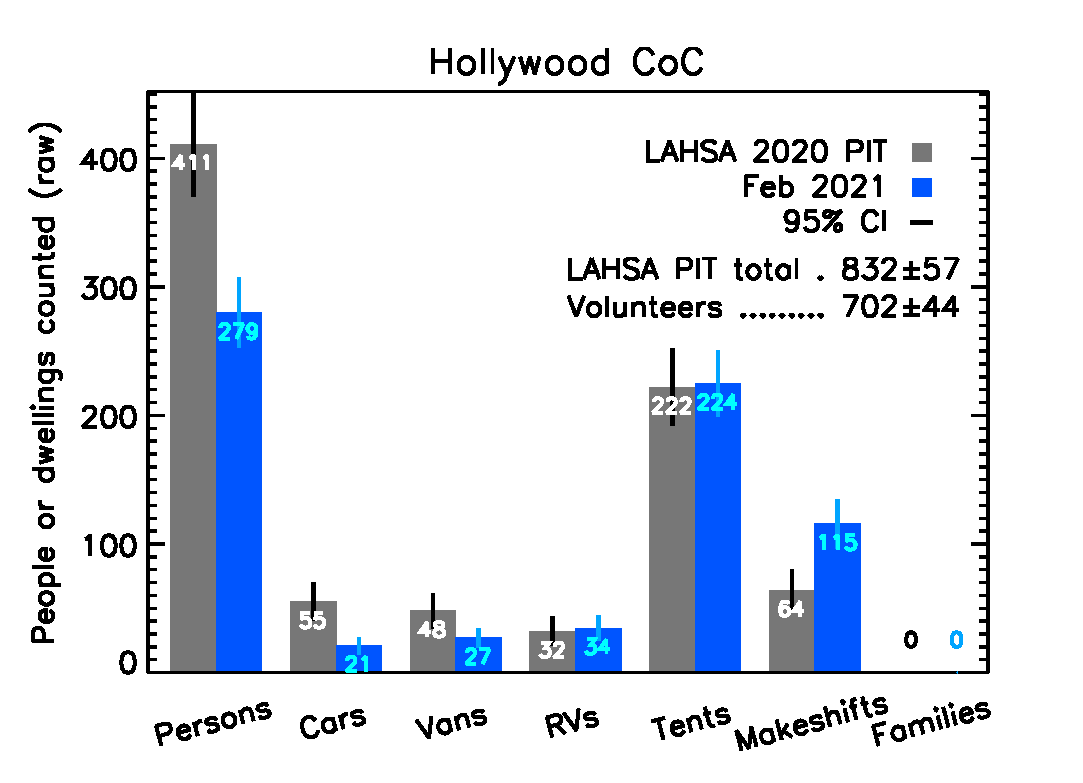
\includegraphics[width = 0.47\textwidth, trim = 1cm 0cm 0cm 0cm]{Hwood2021Bars}
	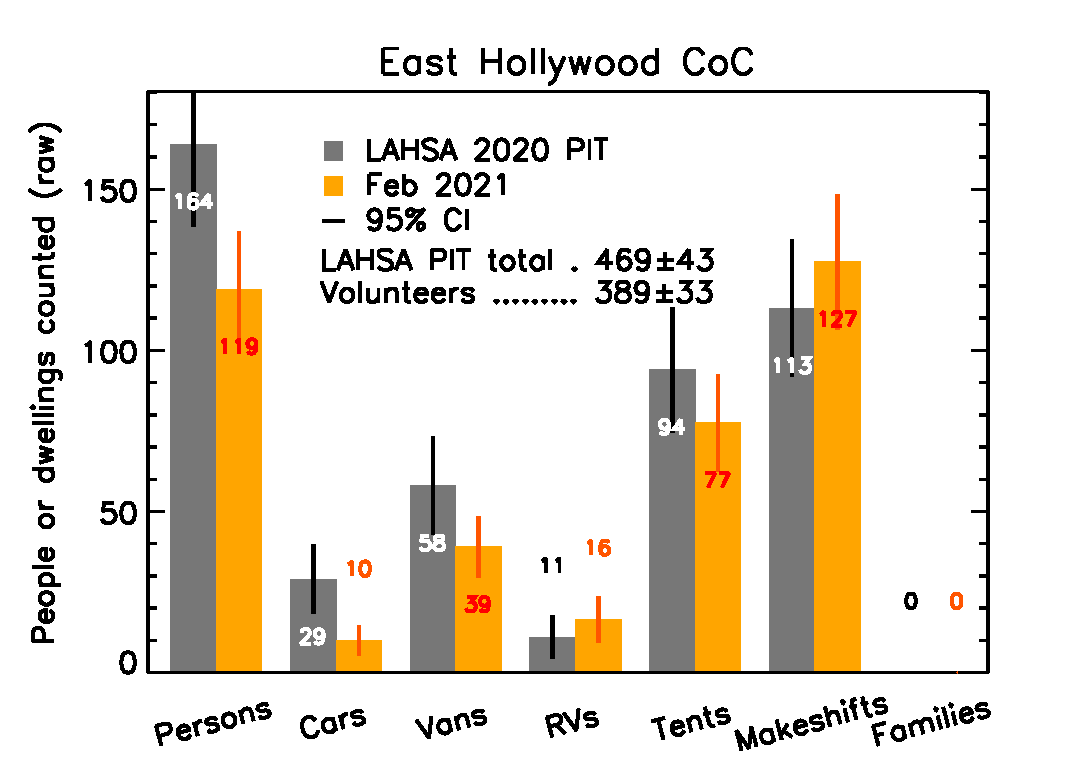
\includegraphics[width = 0.47\textwidth, trim = 0cm 0cm 1cm 0cm]{Eho2021Bars}
	\caption{Raw tallies of unsheltered persons and dwellings in Hollywood and East Hollywood
			(left/right) from the 2020 and 2021 PIT counts (grey/colors). Persons, cars, 
			and vans fell in both communities while RVs and tents stayed statistically flat. 
			Makeshift structures are the only category to show a potential common increase. 
			Overall, we identified 208 fewer people and dwellings compared to 2020,
			with similar 16\% decreases assessed by almost entirely independent teams
			in both communities. ``Persons'' are TAY+Adults.}
	\label{fig:rawCounts}
\end{figure*}

\begin{figure*}[t]
	\centering
	\includegraphics[width =0.47\linewidth, trim = 0.5cm 0cm 0cm 0cm]{hwoodHist}
	\includegraphics[width =0.47\linewidth, trim = 0cm 0cm 0.5cm 0cm]{ehoHist}
	\caption{Explain what the PDFs and CDFs are, what the colors mean.}
	\label{fig:communityPDFs}
\end{figure*}

\subsection{Duplicate Counts}
\label{sec:dupes}

Each volunteer tract in both communities (30) were assigned to at least two independent counting teams.
Four tracts additionally received a third pass. Pass 1 paired tracts by tract number. Pass 2 paired projected 
high-population tracts with one that was geographically nearby. Pass 3 was the same as Pass 1 with 
pairings presented in reverse order, such that teams deployed simultaneously would likely start in different 
tracts. 

Results for one of the two teams assigned to tract 1925.20 could not be interpreted, making it the only
volunteer tract with one population estimate.

Figure \ref{fig:dupeChar} shows intercounter comparisons of raw counts (people+dwellings)
at the tract and category levels. Average offsets are close to Poisson expectations in all cases 
except for the highest occupancy tracts, where they are inflated by an outlier (see below).
Explicitly, $\langle\sqrt{(\nu_{1}-\nu_{2})^{2}/(\nu_{1} + \nu_{2})}\rangle=1.4$, where
$\nu$ is the total number of dwellings and people in a given tract returned by one of the teams. 

The outlier is tract 1901.00, whose repeat measurements differ by $6.6\,\sigma$. There, 
one team counted $\{P,C,V,R,T,M\}=\{23,1,1,1,6,2\}$ while the other counted $\{77,15,10,1,6,6\}$. 
Abramson re-counted this tract on-foot 14 hours after the PIT tally, obtaining $\{36, 4, 6, 0, 8, 2\}$.
In total, this tally ($\nu_{\rm Abramson}=56\pm7$) is within $1.9\,\sigma$ of the volunteers' mean 
($\langle\nu_{\rm PIT}\rangle=75\pm6$). As such, we retain the volunteer PIT estimate as-is. As illustrated in 
Figure \ref{fig:dupeChar}, top, the mean intercounter dispersion drops to $1.3\,\sigma$ if this tract is 
excluded.

In terms of categories, all dispersions are consistent with Poisson expectations except for RVs, where 
agreement is significantly better. Given their salience, this finding is reassuring if unsurprising.

%1901.00 inter-counter difference is 4.7 sigma (sqrt(delta) / root(n1 + n2) / root(2))

%\begin{itemize}
%%	\item All vol tracts counted at least twice;
%%	\item 4 tracts counted 3x;
%%	\item One recount DQed for quality flag (1925.20);
%%	\item Dupe statistics look pretty good. Mean abs discrepancy is consistent
%%		with zero given standard error on mean except for TAY (2.7 sigma) and RVs (3.8).
%%		Normalized differences ($|n_{1}-n_{2}|/\sqrt{n_{1}+n_{2}}$) are a little higher
%%		than $1\sigma$ ($CVRTM=[1.7, 1.1, -, 1.6, 1.4, 0.6, 1.2, 1.6, -]\sigma$), suggesting 
%%		a little more than poisson counting uncertainty, but LEA cross-checked the one
%%		highly discrepant ($\sim$8$\sigma$) tract, 1901.00, and found raw counts consistent
%%		with the average of the two nighttime datasets ($\sim$9:00 AM 26 Feb). 
%	\item Above holds true for 1912.01, which is in Hwood and also a SELAH recount tract. LEA
%		counted 51 totoal ppl/dwellings 12:30 P on 27 Feb vs 51 by vols night of count.
%\end{itemize}

No team counted tracts in both Hollywood and East Hollywood. As such, the volunteer counts
in those communities represent independent datasets. Including the professional-counted tracts, 
cross-talk comes from one tract in East Hollywood counted by a team that surveyed five 
tracts in Hollywood. We discuss intercommunity comparisons between volunteer and 
professionally counted tracts in Section \ref{sec:crossChecks}.

%{\bfr PRO TRACT RAW COUNT SHARE 2020: 44\% (23 tracts)
%
%PRO TRACT RAW COUNT SHARE 2021: 43\% (all tracts)}
%
%{\bfr Barely consistent if all of last year's vans and cars are still here. 95\% confidence limit $996\pm69$ can reach 1065 (v 1058) 
%in Hollywood, $598\pm 59= 657$ vs.\ 656 last yr in E.~Hollywood. BOTH AT 2020 SPA4 WEIGHTS!}


\section{Results}
\label{sec:results}

This section presents community- and aggregate-level estimates for the number of unsheltered people 
living in Hollywood and East Hollywood as of 25 February 2021. Sections \ref{sec:hWood} and \ref{sec:eHo} 
summarize our results, \ref{sec:comp} compares them to the 2020 LAHSA PIT estimates, 
\ref{sec:concentration} quantifies the population's geographic distribution, and \ref{sec:crossChecks}
presents cross-checks.

%Section \ref{sec:discussion} describes how 
%varying elements of Section \ref{sec:mc}'s analysis modulates these results.

\begin{table*}[t!]
\caption{Greater Hollywood 2021 PIT Unsheltered Data and Population Estimates}
\resizebox{\linewidth}{!}{%
\begin{tabular}{lcccccccccc}
\toprule
 & Adult & TAY & Car & Van & RV & Tent & Makeshift & {\bf 2021 Total} & {\bf 2020 Total} & {\bf Difference} \\ \cmidrule{1-11}
{\bf Hollywood} \\ %\cmidrule{1-1}
Counts & 277 & 2 & 21 & 27 & 34 & 224 & 115 & {\bf 702} & {\bf 831} & $\bf -15\%$ \\
Inhabitants & 277 (27) & 2 (5) & 32 (11) & 49 (13) & 50 (14) & 332 (29) & 195 (24) & {\bf 937 (93)} & {\bf 1058} & $\bf -11\%\,(9\%)$\\% (76)
Category share & 30\% (3\%) & 0\% (0\%) & 3\% (1\%) & 5\% (1\%) & 5\% (1\%) & 35\% (3\%) & 21\% (3\%) & -- & -- & -- \\ \cmidrule{1-11}
{\bf East Hollywood} \\ %\cmidrule{1-1}
Counts & 114 & 4 & 10 & 39 & 16 & 77 & 127 & {\bf 389} & {\bf 469} & $\bf -17\%$ \\
Inhabitants & 114 (19) & 4 (4) & 15 (8) & 70 (15) & 24 (9) & 115 (19) & 216 (23) & {\bf 557 (83)} & {\bf 656} & $\bf -15\%\,(12\%)$\\% (60)
Category share & 20\% (3\%) & 1\% (1\%) & 3\% (1\%) & 13\% (3\%) & 4\% (2\%) & 20\% (3\%) & 39\% (4\%) & -- & -- &--
\\ \bottomrule
\end{tabular}
}
\caption*{Parentheses denote 90\% uncertainties (binomial in the case of the categories). 
Uncertainties larger than estimates imply that only upper limits are available. Marginalized
upper limits are obtainable from the results file and imply $<$3 unaccompanied minors and
$<$3 unsheltered families in either community.}
\label{tbl:summary}
\end{table*}


\subsection{Hollywood}
\label{sec:hWood}

Counters identified $702\pm44$ (95\% CI) persons and dwellings in the 21 census tracts 
comprising the Hollywood Community. Modulated by the baseline CVRTM weights, these 
estimates imply a total unsheltered population of $936\pm92$ people 
(90\% CI; Figure \ref{fig:communityPDFs}, left), with the plurality (35\%) living in tents 
(Table \ref{tbl:summary}; Figure \ref{fig:rawCounts}, left). The five tracts counted by professional 
teams---largely along the US 101 corridor---comprised 42\% of raw counts and 43\% of inferred 
unsheltered people. Tract 1910.00 (pro-counted) had the most people and dwellings ($123\rightarrow170$
total population); 1899.03 had the fewest ($0\rightarrow$$<$12 total population). %These tracts also bracket the population statistics. 


\begin{figure*}[]
	\centering
	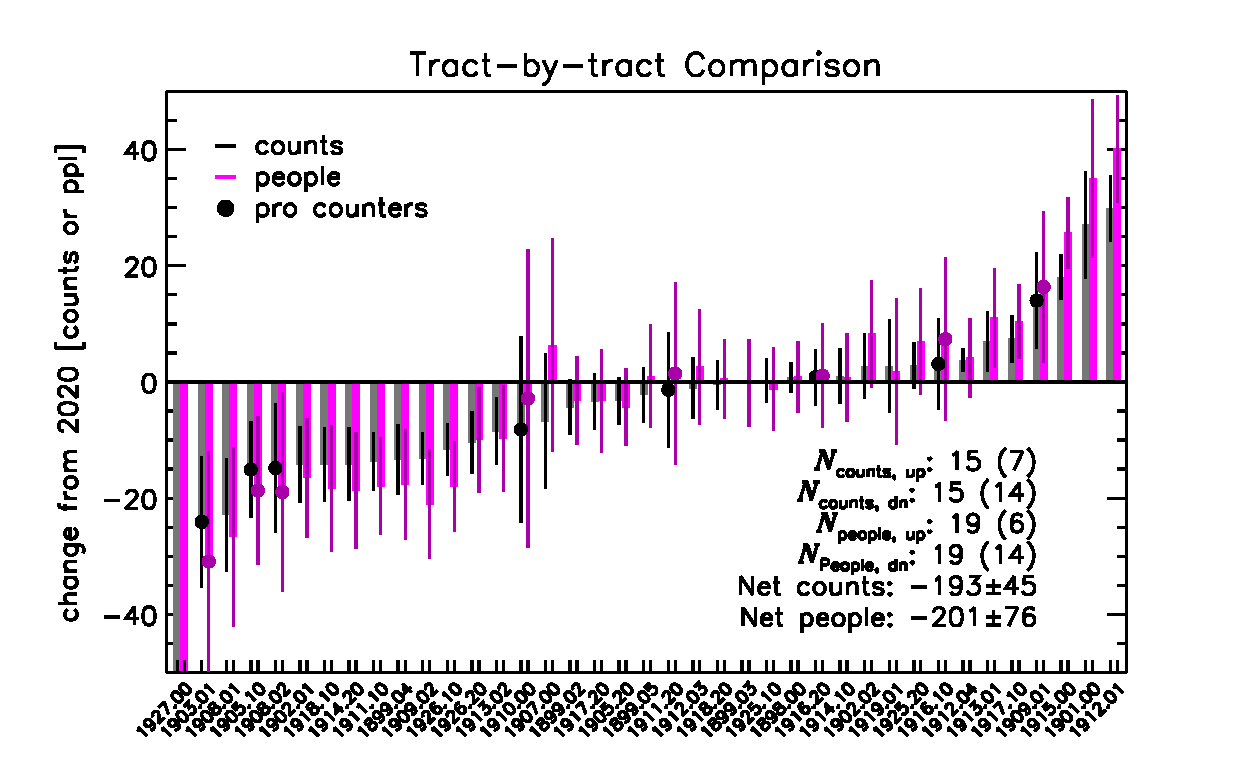
\includegraphics[width = 0.8\linewidth, trim = 0cm 0cm 0cm 0cm]{tractsYrYr}
	\caption{Tract-level year-on-year changes. Pro and vol trends are similar. Net loss of
			about 200 people or identified persons+structures. 1927.00 saw the biggest
			loss, which is explainable via XYZ.}
	\label{fig:tractYrYr}
\end{figure*}

Modifying the CVRTM weights from the baseline SPA4/CD13 values to their SPA4 wide values 
lowers Hollywood's inferred total unsheltered population to $912\pm68$ people; applying
an updated tent weight based on a survey in Hollywood raises it to $944\pm118$ people (Section
\ref{sec:discussion}). Neither represents a significant change from baseline.

\subsection{East Hollywood}
\label{sec:eHo}

Counters identified $389\pm33$ (95\% CI) persons and dwellings in the 18 census tracts 
comprising East Hollywood. Modulated by the baseline CVRTM weights, these estimates imply 
a total unsheltered population of $556\pm83$ people (Figure \ref{fig:communityPDFs},
right), with the plurality (39\%) living in makeshift structures (Table \ref{tbl:summary}, 
Figure \ref{fig:rawCounts}, right). The four tracts counted by professional teams comprised 46\% of 
those counts and 47\% of inferred unsheltered people. Tract 1927.00 (pro-counted) had the 
most people and dwellings ($87\rightarrow129$ total population); 1912.04 had the fewest 
($5\rightarrow$$<$16 total population). 
%These tracts also bracket the total population statistics. 
%The plurality of counts were of makeshift structures---statistically 
%consistent with the number of persons identified on the street---followed by tents 
%(Figure \ref{fig:rawCounts}, right).

Modifying the CVRTM weights from the baseline SPA4/CD13 values to the SPA4 wide values 
lowers East Hollywood's inferred total unsheltered population to $539\pm59$ people; applying
the updated tent weight raises it to $559\pm87$ people. Neither represents a significant change from 
baseline.

\begin{figure*}[]
	\centering
	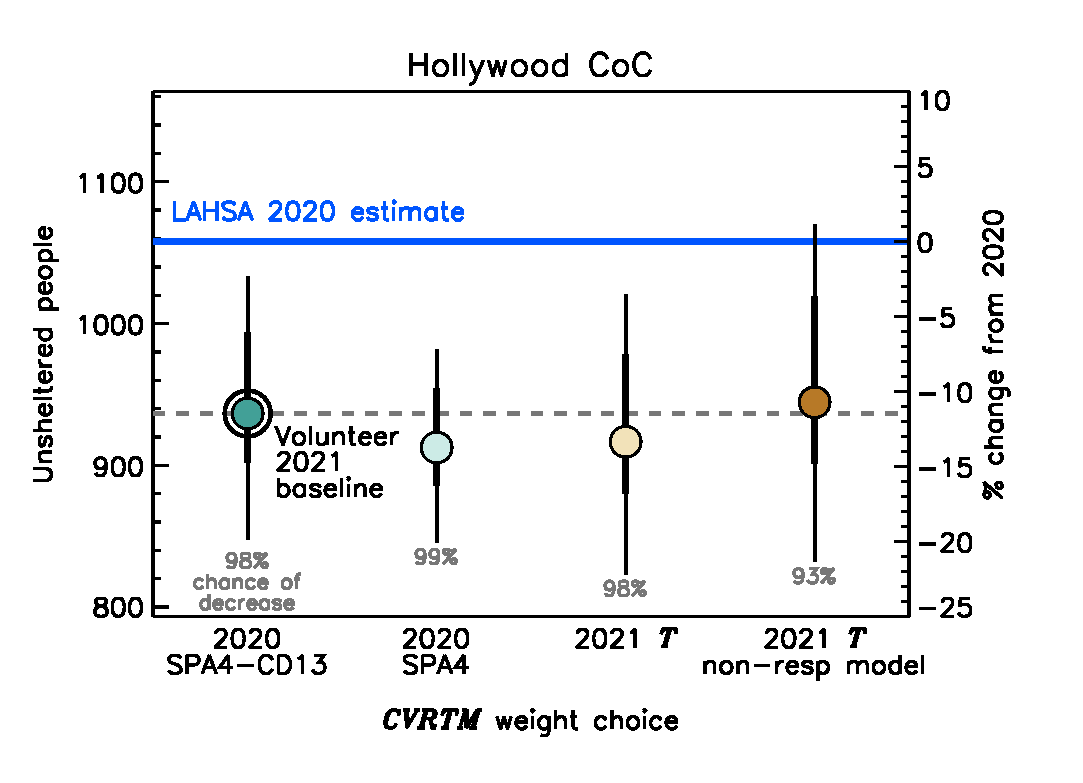
\includegraphics[width = 0.48\textwidth, trim = 0cm 0.5cm 0cm 0cm]{hwoodFinal}
	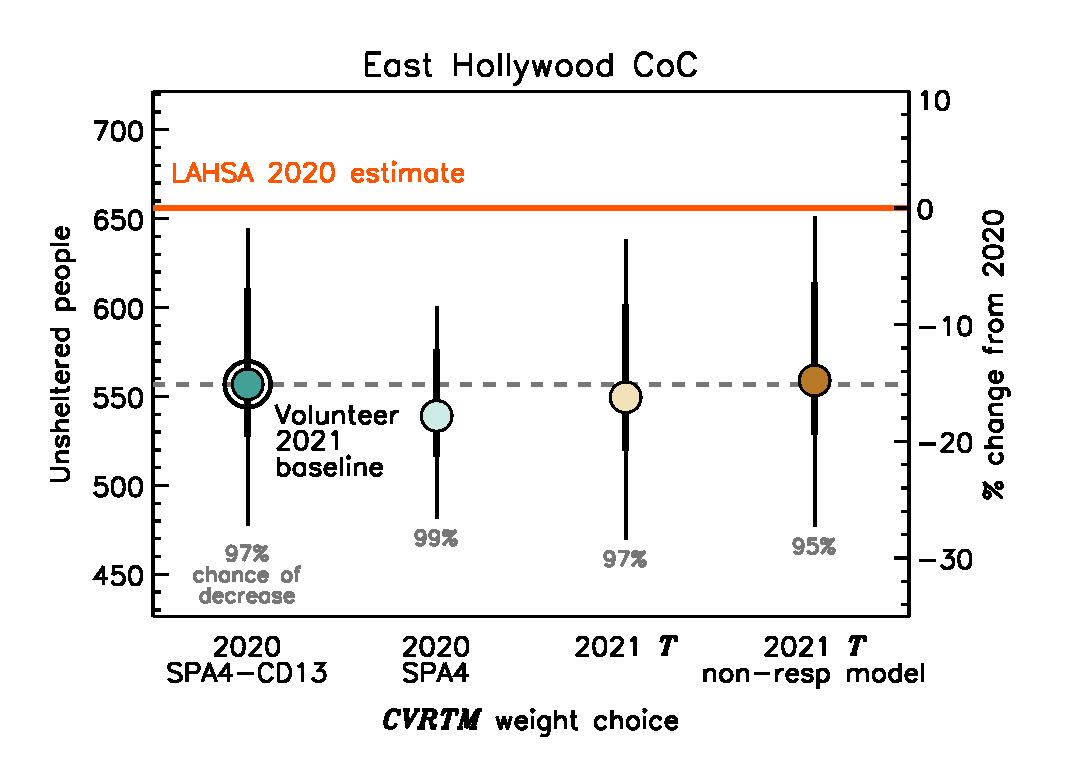
\includegraphics[width = 0.48\textwidth, trim = 0cm 0.5cm 0cm 0cm]{ehoFinal}	
	\caption{Unsheltered populations in Hollywood (left) and East Hollywood (right) 
			as functions of CVRTM weights. The baseline estimate uses the same weights as the 
			2020 LAHSA Community Summaries. Using SPA4 weights or replacing the tent 
			weight, $T$, with results from a survey conducted in Hollywood yields consistent
			results. All imply at least a 93\% chance that unsheltered homelessness has fallen
			by some amount, with likely declines of $12\%\pm9\%$ and $15\%\pm12\%$
			in Hollywood and East Hollywood, \resp.}
	\label{fig:wtComp}
\end{figure*}


%\begin{figure}[]
%	\centering
%	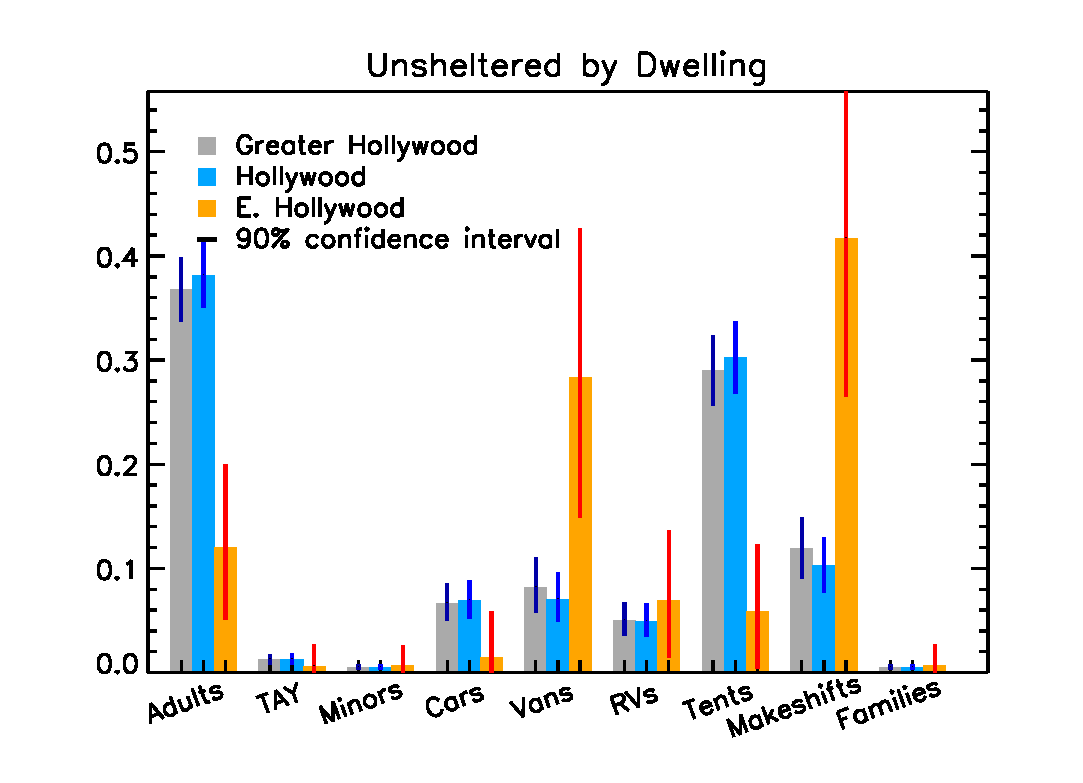
\includegraphics[width =\linewidth]{allTracts/allBreakdownBar}
%	\caption{}
%	\label{fig:popFracs}
%\end{figure}

\subsection{Comparison to 2020}
\label{sec:comp}

The official LAHSA estimates from the 2020 PIT count are overplotted in Figure \ref{fig:communityPDFs} 
as red vertical lines in each panel: 1058 unsheltered people in Hollywood, 656 in East Hollywood.
Our baseline inferences suggest a $>$95\% probability that the current population has fallen from 
those levels. Using the median and 90\% CI, we infer declines of $11\%\pm9\%$ and $15\%\pm12\%$, \resp. 

Figure \ref{fig:tractYrYr} shows the changes in counts and inferred population in each tract 
geographically illustrated in Figure \ref{fig:map}. In total, we find significant gains in 7 (6)
tracts in terms of counts (people), and significant declines in 14, resulting in net changes of $-193\pm45$
and $-201\pm76$ counts or people, \resp.\footnote{These estimates incorporate uncertainties 
from backing-out tract-level CVRTM counts from their total populations and person counts provided
by the LAHSA data portal.}

The tracts with the largest year-on-year gain (1912.01, $+40$ people) and loss (1927.00, $-125$ people)
are both in East Hollywood. They contain Barnsdall Park and US 101, \resp. 

%We speculate as to why these 
%tracts, specifically, saw such changes in Section \ref{sec:discussion}, along with why counts of rough
%saw particularly large declines.

Given the deficit in raw counts, it seems unlikely that reasonable modifications to the CVRTM weights 
will qualitatively change the trend we infer. The $w_{T}$ and $w_{M}$ weights are the largest potential error 
sources due to the high proportion of people living in tents and makeshifts. To constrain their evolution
from last year, \href{https://selahnhc.org}{SELAH} outreach teams surveyed 47 tents (38 responses) 
in Hollywood on 28 Feb. This exercise yielded a mean occupancy of $w_{T}=1.39\pm0.14$ people per tent, 
or $w_{T}=1.50\pm0.22$ when non-responses are modeled.\footnote{We assumed they were equally likely to have anywhere 
from 0 to 4 occupants, each.} While neither the full 2021 PIT area nor $w_{M}$ has been assessed, the 
above values are consistent with the official 2020 weight of $w_{T}=1.48\pm0.11$. 

Figure \ref{fig:wtComp} illustrates the effect of the above CVRTM modifications. In all cases, we infer at 
least a 93\% chance of a decline compared to the 2020 PIT count.

We encourage robust efforts to update the CVRTM weights, but the changes needed to null the 
decline we infer from 2020 are substantial. Only changes to $w_{T}$ and $w_{M}$ can reasonably 
achieve it, and must rise to 2.2 and 2.6 people from 1.5 and 1.7 people, \resp, in 2020. Not withstanding
the above survey, such $\sim$50\% increases in {\it mean} occupancies seem unlikely, especially as
known COVID-related tent distribution efforts have pushed in the opposite direction (Section 
\ref{sec:discussion}). While 2021 is unprecedented in many ways, historically, no SPA4/CD13 
CVRTM weight has changed by more than $\sim$30\% year-on-year since 2018 
($w_{R}$ fell from $\sim$2 to $\sim$1.4 from 2019 to 2020).

All of the above is largely a reflection of the fact that persons seen on the street fell by $\sim$30\%
(Figure \ref{fig:rawCounts}). Cars and vans are also down from last year by more than the number of 
safe parking spaces (Section \ref{sec:discussion}), with only makeshift structures showing a potential 
common gain. All told, the total number of dwellings remained flat in most tracts. Although uncertainties 
in East Hollywood are large, Figure \ref{fig:proVolComp} reveals these trends to be common across 
communities and tracts counted by volunteers or professionals. Such consistencies in nearly independent 
datasets suggest the results are robust. Section \ref{sec:crossChecks} presents further cross-checks.

%(Unsheltered people make up 3.5\% of tract 1907.00's total population, according to 2020 estimates
%from the US Census.)
%combined with COVID-related relaxations of tent-folding ordinances and the de-scoping of
%sanitation efforts suggests that the 

\subsection{Geographic Concentration}
\label{sec:concentration}

Everyday experience (and {\bfr maybe another map}) confirms that unsheltered homelessness is
unevenly distributed. However, given the role of public opinion in policymaking, it is worth 
providing empirical grounding for arguments over, e.g., the placement of new permanent supportive 
housing (PSH) facilities by quantifying that statement. Figure \ref{fig:gini} is one attempt to do so. 

Combining our PIT \Count\ results with 2020 
\href{https://geomap.ffiec.gov/FFIECGeocMap/GeocodeMap1.aspx}{US Census} 
data, we can compare the distribution of unsheltered Angelenos vs.\ all Angelenos in Greater
Hollywood. The top panel shows simply the fraction of inhabitants in a given tract that we
identified as unsheltered. This fraction spans $\sim$0\% to over 4\%, with a mean around 
1\%---40\% higher than the \href{https://www.lahsa.org/documents?id=4680-2020-greater-los-angeles-homeless-count-city-of-los-angeles}{LA's global unsheltered fraction} as of Jan.~2020.

The bottom panel plots the cumulative contribution of each tract to Greater Hollywood's
total and unsheltered populations. If people were equitably distributed, the curves would 
correspond to a diagonal line with unit slope, yielding a Gini coefficient $c_{\rm Gini}=0$. 
The total population in Greater Hollywood has $c_{\rm Gini}\simeq0.1$---50\% of people 
living 40\% of tracts---close to evenly distributed. The unsheltered population, 
on the other hand, has $c_{\rm Gini}=0.44\pm0.02$---50\% of people living in 20\% of 
tracts---analogous to those describing income inequalities in 
\href{https://en.wikipedia.org/wiki/List_of_countries_by_income_equality#UN,_World_Bank_and_CIA_list_\%E2\%80\%93_income_ratios_and_Gini_indices}{Rwanda, Philippines, or Malawi} 
as estimated by the World Bank. Such a concentration of lived trauma, real poverty, and the
attendant externalities of unsheltered homelessness should condition the design of policies
and the thoughts of policymakers holding equity as a core value.

\begin{figure}[t]
	\centering
	\includegraphics[width =\linewidth, trim=0.75cm 0cm 0cm 0cm]{volProfComp}
	\caption{Comparison of trends in pro- and vol-counted tracts in both communities.
			Consistency is good, though 1927.00 counts for a lot. We haven't
			broken down the 2020 results at the tract+CVRTM level yet.}
	\label{fig:proVolComp}
\end{figure}

\begin{figure}[t]
	\centering
	\includegraphics[width =\linewidth, trim = 0cm 0cm 0cm 0cm]{totPopFrac}\\
	\includegraphics[width =\linewidth, trim = 0cm 0.5cm 3.5cm 0.25cm]{gini}
	\caption{All tracts in Greater Hollywood. This Gini Coefficient
			is about the same as 
			\href{https://en.wikipedia.org/wiki/List_of_countries_by_income_equality}{Kenya's}.
			50\% of unsheltered persons and dwellings are concentrated in 20\% of census
			tracts.}
	\label{fig:gini}
\end{figure}

\subsection{Cross-checks}
\label{sec:crossChecks}

Multiple cross-checks involving independent counters and external datasets suggest 
that the raw counts from our 2021 PIT \Count\ are accurate. The validating data are also
available at {\bfr website}.

\subsubsection{Internal checks}

First are Figure \ref{fig:dupeChar}'s inter-comparisons of the count's 37 duplicate tract 
measurements, suggesting per-tract and -category counting uncertainties are consistent with  
the random errors built into the analysis. There is thus no evidence that counters were biased in
identifying unsheltered persons or dwellings. Such data do not preclude the possibility of systematic 
inefficiencies in identifying, e.g., cars and vans---which can be difficult at night---but 
Figure \ref{fig:proVolComp}'s illustration that at least person and dwelling trends are consistent 
in tracts counted by volunteers and professionals---who surveyed on foot in daylight---suggests 
that such biases are probably not large. Post-facto independent measurements of key geographies
suggest this, too.

\subsubsection{External checks}

Three census tracts were re-surveyed in detail, none of which yield evidence of a PIT undercount:
\begin{itemize}
	\item Tract 1901.00: intercounter variability outlier. Abramson
		  assessed this tract 14 hours after the PIT count (circa 9:00 AM) with results 
		  $1.9\,\sigma$ {\it lower} than the volunteers' average.
	\item Tract 1912.01: largest increase. Abramson assessed this tract on 
		27 Feb.\ circa 12:00 PM. Results were consistent with the PIT \Count\ to within 
		$1\,\sigma$.
	\item Tract 1927.00: largest decrease. Abramson assessed this tract
		on 4 March circa 8:30 AM by vehicle with results lower than the PIT's assessment. 
		However, given this tract's density and configuration---home to many freeway ramps and
		shoulders---it was originally surveyed on foot by outreach professionals. As such, A bramson's 
		vehicular recount only suggests that the PIT data are not biased so as to induce an artificial decline.
\end{itemize}

Two larger-geography surveys concur quantitatively and qualitatively:
\begin{itemize}
	\item Biweekly data from \href{https://hollywoodpartnership.com/}{\it The Hollywood Partnership} 
		from 19 Feb.\ are consistent with PIT data in a common tract (1902.02) and with an independent 
		recount of the entire Business Improvement District's geography performed 28 Feb.\ by Abramson and 
		Kohan. These data also imply a decline from past values.
	\item Three tracts in Echo Park and Silver Lake monitored biweekly by SELAH since May 2020 
		also show similar declines. 
\end{itemize}
%
%A 27 Feb.\ recount of tract 1912.01 in East Hollywood conducted as as part of a
%		\href{https://selahnch.org}{SELAH} monitoring campaign agrees with our PIT value.% in unsheltered homelessness.
%

Finally, safe parking---a known sink---provides 49 spaces in or near the survey area (Hollywood,
East Hollywood, and Echo Park). If occupied on 25 Feb., these locations probably went uncounted.
That suggests $80\pm16$ total car and van dwellers should be added to our results (assumes 
equal mix). If so, the baseline chance of a decline from 2020 falls from 98\% to 92\%.

All of the above suggests that our results are reliable.
%Assumes equal mix of cars + vans.
%From Starkey: Hwood = 25, Eho = 10, EchoPk = 14; total = 49; total CD13 = 59 but I think it's reasonable
%to truncate at Echo Pk. It's 90% if you include all 59 spaces.

%		   P	C     V	    R	 T     M
%1901.00 -- 50    8    5.5   1     6      4 -- 2021, raw
%1901.00 -- 36    4     6     0     8      2 -- 26 Feb ABRAMSON 9.00 AM
%
%1927.00 -- 48    1      5     0    53    70 -- 2020, raw
%1927.00 -- 20    0     0     7     6     54 -- 2021, raw
%1927.00 -- 15     0     9     5    14    21 -- 4 Mar 2021 ABRAMSON 8.45 AM
%
%1912.01 --  18.5  0.5  3.5  1.5  5.5  12 -- 2021, raw
%1912.01 --  21     0      4     1     8      6  -- 27 Feb ABRAMSON 12.15 PM
%
%1902.02 -- 9      --     --     --     8   5.5 -- 2021, raw
%1902.02 -- 9      --     --     --    17    --  -- BID 2/19

% 1907.00 is also interesting in that total population stayed nearly the same but identified
% individuals and dwellings basically swapped: IND 73->38; CVRTM 31->70. This has a big impact
% on people's perceptions, and it's in a very high-traffic part of the community.

%The pro/vol trends are consistent everywhere except tract 1927.00, 
%			where pro counts dropped significantly more for both individuals and dwellings (esp.\ 
%			tents). 1927.00 comprises 22\% of total counts in East Hollywood. Unsheltered 
%			homelessness in that CoC was flat or rose slightly outside of that tract.}
%{\bfr 1927.00 is the tract with the PATH Madison PSH. Phase II opened in Jan 2020---leasing began May 
%2020---and is 120 units, some of which were filled from nearby folks but I dunno how many. LEA recounted 
%this tract 4 March at $\sim$9:00 AM and found 94 total population vs.\ pro's 129. Only place where
%LEA counted more objects was vans. Adding that to the pro total adds 16 people (9 vans).

%HOLLYWOOD -- Zero delta requires CVRTM mean occupancies of:\\
% - 5.00 ppl/car (from 1.51)\\
% - 5.00 ppl/van (from 1.77)\\
% - 4.95 ppl/RV (from 1.42)\\
% - 2.03 ppl/tent (from 1.48)\\
% - 2.73 ppl/mkshft (from 1.68)\\
%
%EAST HOLLYWOOD -- Zero delta requires CVRTM mean occupancies of:\\
% - 5.00 ppl/car (from 1.51)\\
% - 4.33 ppl/van (from 1.77)\\
% - 5.00 ppl/RV (from 1.42)\\
% - 2.78 ppl/tent (from 1.48)\\
% - 2.45 ppl/mkshft (from 1.68)

% ------ SUMMARY for HWOOD ------ 
%
%Total People (90%CI) .   936+/-92
%Fraction vs. last yr .   0.89+/-0.09
%Total counts..........   702
% > Adults    : 277 (39%), 277, (29%)
% > TAY       :   2 ( 0%),   2, ( 0%)
% > Minors    :   0 ( 0%),   0, ( 0%)
% > Cars      :  21 ( 2%),  31, ( 3%)
% > Vans      :  27 ( 3%),  47, ( 5%)
% > RVs       :  34 ( 4%),  49, ( 5%)
% > Tents     : 224 (31%), 330, (35%)
% > Makeshifts: 115 (16%), 193, (20%)
% > Families  :   0 ( 0%),   0, ( 0%)
%% Compiled module: MINMAX.
%Min/max ppl/tract ..... 0, 169
%Min/max counts/tract .. 0, 123
%
% ------ SUMMARY for EHO ------ 
%
%Total People (90%CI) .   556+/-83
%Fraction vs. last yr .   0.85+/-0.13
%Total counts..........   389
% > Adults    : 114 (29%), 114, (20%)
% > TAY       :   4 ( 1%),   4, ( 0%)
% > Minors    :   0 ( 0%),   0, ( 0%)
% > Cars      :  10 ( 2%),  14, ( 2%)
% > Vans      :  39 (10%),  68, (12%)
% > RVs       :  16 ( 4%),  23, ( 4%)
% > Tents     :  77 (19%), 114, (20%)
% > Makeshifts: 127 (32%), 214, (38%)
% > Families  :   0 ( 0%),   0, ( 0%)
%Min/max ppl/tract ..... 6, 129
%Min/max counts/tract .. 5, 87

\section{Discussion}
\label{sec:discussion}

\begin{figure}[t]
	\centering
	\includegraphics[width =\linewidth, trim = 1cm 0.5cm 0cm 0cm]{tract1907comp}
	\caption{Illustration of what's happened in 4 tracts---persons and structures
			swapping prominence---in this case with the total population
			$\sim$conserved. This is also an example of one of 5 tracts where
			dwelling frequencies at least doubled. 1907 happens to be in the 
			heart of Central Hollywood, increasing the visual impact of this
			rise in dwellings.}
	\label{fig:1907}
\end{figure}

The upshot of the above is that, as far as we can assess, the number of people experiencing unsheltered
homelessness in Greater Hollywood has declined to levels slightly above those in 2019 (917 and 491 people in 
Hollywood and East Hollywood, \resp). A number of factors may contribute to this change, some 
COVID-related and some not.

\subsection{Government Initiatives}

Foremost among these are government programs aimed at moving people indoors and staunch inflow into 
homelessness. The two most salient are COVID-related: Project Roomkey and city and state eviction moratoria.
%Note that Coordinate Entry System (CES) data will constrain all of the following scenarios.

\subsubsection{Eviction Moratoria}

We have no data on how many people the latter has prevented from becoming unhoused. However,
per the LAHSA Count report, nearly 83,000 people became unhoused in 2020 from LA County's pool 
of over half a million rent-burdened residents. Of these, $\sim$7500 could not be rehoused. Thus, if the eviction
moratoria were capable of reducing even 10\% of last year's inflow, extant mechanisms may have had the 
capacity to place everyone under a roof.

\subsubsection{Project Roomkey}

More information is accessible regarding Project Roomkey (PRK). Also according to the 2020 Count report, 
over 6000 unhoused LA County residents became sheltered between March and May of that year.
Examining only \href{https://www.lahsa.org/documents?id=4672-2020-homeless-count-council-district-13}
{CD13's} share of \href{https://www.lahsa.org/documents?id=4585-2020-greater-los-angeles-homeless-count-los-angeles-continuum-of-care-coc-}{LA County's unsheltered senior population} (6.5\%), perhaps 100 of PRk's 
\href{https://projectroomkeytracker.com/}{1608 occupied rooms} were filled with Greater Hollywood residents 
on the night of 25 Feb. If so, this would account for about half the inferred global reduction.

Data from the Coordinated Entry System (CES) will constrain this scenario.

\subsubsection{A Bridge Home}

Unrelated to COVID, at least one \href{https://www.lamayor.org/ABridgeHome}{\it A Bridge Home} (ABH) site 
opened in Los Feliz between this year's grassroots and last year's official PIT count. The catchment area for this ABH's
100 beds spans nearly all of Greater Hollywood. Assuming a 50\% occupancy reduction due to COVID precautions,
this site can account for a further 50 people exiting the unsheltered population.

Of course, ``decompression'' of congregate living sites due to COVID simultaneously reduces the occupancy of extant 
shelters. Again assuming 50\% reductions in beds, we estimate that the five ABHs \href{https://arcg.is/0fy81}
{whose catchments touch Greater Hollywood}---Schrader, YWCA/Lodi (recently expanded), Gardner, Riverside, and 
Lafayette---to have contributed a net addition of 33 beds (398 total, 116 new, 83 lost to decompression). However,
{\it locally}, the addition can be substantially larger. Indeed, tract 1927.00 overlaps with three ABHs, two of which 
were new. In that tract, as many as 89 beds may have come online---excluding the contribution from a known new
PATH permanent supportive housing site (see below).

CES data will constrain this scenario.

\subsubsection{Permanent Supportive Housing}

Finally, 120 PATH permanent supportive housing (PSH) units may also have contributed. While all of those units did not 
go to local residents, the site is located in tract 1927.00---that which saw the largest year-on-year decline from 2020. Any 
units that {\it did} go to locals would help drive that tract's large observed decrease, along with the potential 89 new
ABH beds just discussed. 

CES data will constrain this scenario.

\subsection{Other Losses}

\subsubsection{Geographic Leakage/Edge Effects}

Due to limited resources, our PIT \Count\ could only cover a limited geography. As such, an obvious potential source
of population loss is people exiting Greater Hollywood to nearby communities. In border tracts, this would entail nothing
more than moving across the street. Tract 1927.00 is, again, special in this regard as it has two borders to other communities.
There is also a substantial community of unsheltered Angelenos opposite its eastern edge. We cannot exclude this possibility,
though additional upcoming grassroots PIT events in Mid City and Silver Lake---which bound Greater Hollywood to the
southwest and east, \resp---may provide insights.

\subsubsection{Deaths}

An unfortunate but inevitable source of population loss is death. While COVID is perhaps the most salient potential killer,
and while people experiencing homelessness---especially unsheltered---are far more likely to die from COVID than housed
people, \href{http://publichealth.lacounty.gov/media/coronavirus/docs/SummaryReport_People_Experiencing_Homelessness.pdf}
{Dept.\ of Public Health statistics} suggest that $\sim$200 unhoused LA County residents had succumbed to the 
disease by the time of the PIT count. If so, even if that figure is inaccurate by substantial factors, it is not likely to be the
dominant cause of death.

Instead, \href{http://publichealth.lacounty.gov/chie/reports/HomelessMortality2020_CHIEBrief_Final.pdf}, particularly methamphetamine, are likely to dominate. Based on data spanning only the first seven months of 2020, overdoses had
killed 929 people experiencing homelessness---a rate 7.6$\times$ higher than COVID to that point.

All told, deaths of people experiencing homelessness increased by 26\% from January through July, 2020 over the same
interval in 2019. A more rigorous analysis is needed to determine the extent to which these statistics contributed 
qualitatively to the decline we infer, but, quantitatively, they must.

\subsubsection{Phantom Tents}



\subsection{Objective Support for Subjective Trends}

The authors of this report did not expect to discover a decline in Greater Hollywood's unsheltered population.
The ``felt'' condition of homelessness we accumulated over the course of 2020 was one of a meaningful,
if not dramatic worsening. The PIT data provide some hints as to ways to reconcile these subjective and 
objective conclusions.

Principally, smaller scales tell different stories than the community level results. Seven tracts saw at least a 
50\% increase in the number of dwellings. Of these, five saw more than 100\% gains.\footnote{Tracts 1902.02, 
1907.00, 1912.01, 1915.00, 1925.20, accounting for nearly 10\% of all street dwellings and 17\% of all counts.} 
Tracts 1907.00 and 1912.01 are two such notable tracts.

Tract 1907.00 is located in the heart of Central Hollywood's commercial district,\footnote{It spans Fountain Ave to 
Sunset Blvd to Franklin Ave, Vine St to Highland Ave to La Brea Ave.}.  It is one of four tracts wherein the number
of dwellings and persons swapped in rank order compared to 2020. Indeed, the swap was so precise in 1907.00
as to nearly conserve the total number of identified people+dwellings (Figure \ref{fig:1907}). This phenomenon would 
increase the {\it visual salience} of unsheltered living even as the population as a whole remained unchanged.

Meanwhile, tract 1912.01's population did {\it not} remain the same, but more than tripled, leading to the largest 
overall gain vs.~2020. This tract contains the western edge of Vermont Ave between Fountain Ave and Hollywood
Blvd, and the southern edge of Hollywood Blvd between Vermont and Normandie (Barnsdall Park). Both are
are high-traffic corridors and so areas of enhanced visibility. A doubling of tent counts there might have therefore
have an outsized psychological impact.

%Ancillary data from regularly monitored census tracts suggests that the date offset is unlikely to substantially 
%erode comparability between this and past datasets. Limited daytime recounts also suggest that 
%time-of-day effects are sub-dominant.

%1927.00 is actually in the catchment of 3 ABHs that were either new or expanded between PIT counts. 
%Lodi, however, did not fill its new beds, and Lafayette doesn't cover the whole tract, so we won't speculate.
%Nevertheless, technically, even at 50\% decompression, residents of 1927.00 may have been eligible 
%for any of 89 new ABH beds. It's also on the CoC boundary.

\subsection{Quality of Life Degradation}

{\it However}, to say nothing of the implications of the above for conditions after the eviction moratoria
lapse, if there are fewer people on the street today, their quality of life has degraded markedly. COVID has restricted or 
eliminated access to restaurant and park bathrooms, libraries (and so 
\href{https://www.lapl.org/homeless-resources/the-source}{\it The Source} service days), DPSS 
(EBT, Medi-Cal), DMV (ID replacement), and DMH facilities. Physical limitations on caseworker 
access to clients at hospitals and clinics has also hindered successful discharges. These qualitative harms are reflected 
by a 25\% increase in 
\href{https://www.latimes.com/california/story/2021-01-07/the-powerful-synthetic-opioid-fentanyl-is-behind-rising-deaths-in-the-homeless-population}{overdose deaths}, and visually amplified by a doubling of unsheltered dwellings in 13\% of census 
tracts\footnote{Including 1907.00, Central Hollywood's commercial core.} as enforcement of tent folding ordinances
(LAMC 56.11) and City and State sanitation programs were simultaneously 
\href{https://clkrep.lacity.org/onlinedocs/2020/20-0147_misc_3-17-20_p.pdf}{suspended or de-scoped}. 
So, while the PIT data may support the efficacy of programs designed to reduce street 
homelessness, they do {\it not} suggest that the state of homelessness in Greater Hollywood has improved. In the 
fight to rebuild lives---as well as build homes---that fact must remain paramount.


{\bfr 1907.00 people and tents switched. Total unsheltered $\sim$constant but visual perceptions
in this most-highly trafficked tract will make it *feel* like homelessness has increased by a lot.}



\section{Summary}
\label{sec:summary}

Data from February 25, 2021 censuses of Hollywood and East Hollywood shows that 
unsheltered homelessness has fallen in those communities by $11\%\pm9\%$ and 
$15\%\pm12\%$, \resp, compared to the 2020 LAHSA Point-In-Time (PIT) count (90\% CI). 
A 30\% drop in individuals seen on the street drives this change, reducing the number of identified 
persons and dwellings in about a third of census tracts. Unsheltered living is thus likely to have 
declined quantitatively even if the average occupancy of, e.g., tents is updated. Simultaneously, 
however, 13\% of tracts saw at least a doubling in street dwellings. This trend may contribute to 
qualitative perceptions that the state of homelessness has worsened over the past year, which---given 
COVID-related reductions in health, hygiene, and social support services---are also likely to be accurate.
Coordinated Entry System data will reveal whether homelessness has declined in toto or if 
government initiatives reduced only the portion of people living unsheltered in Greater Hollywood.

\section*{}

LA acknowledges Dan Kelson for his analysis insights and all of the volunteers who participated
in the 2021 grassroots PIT \Count.

\appendix

\section{Example Documents}

\begin{figure*}
	\centering
	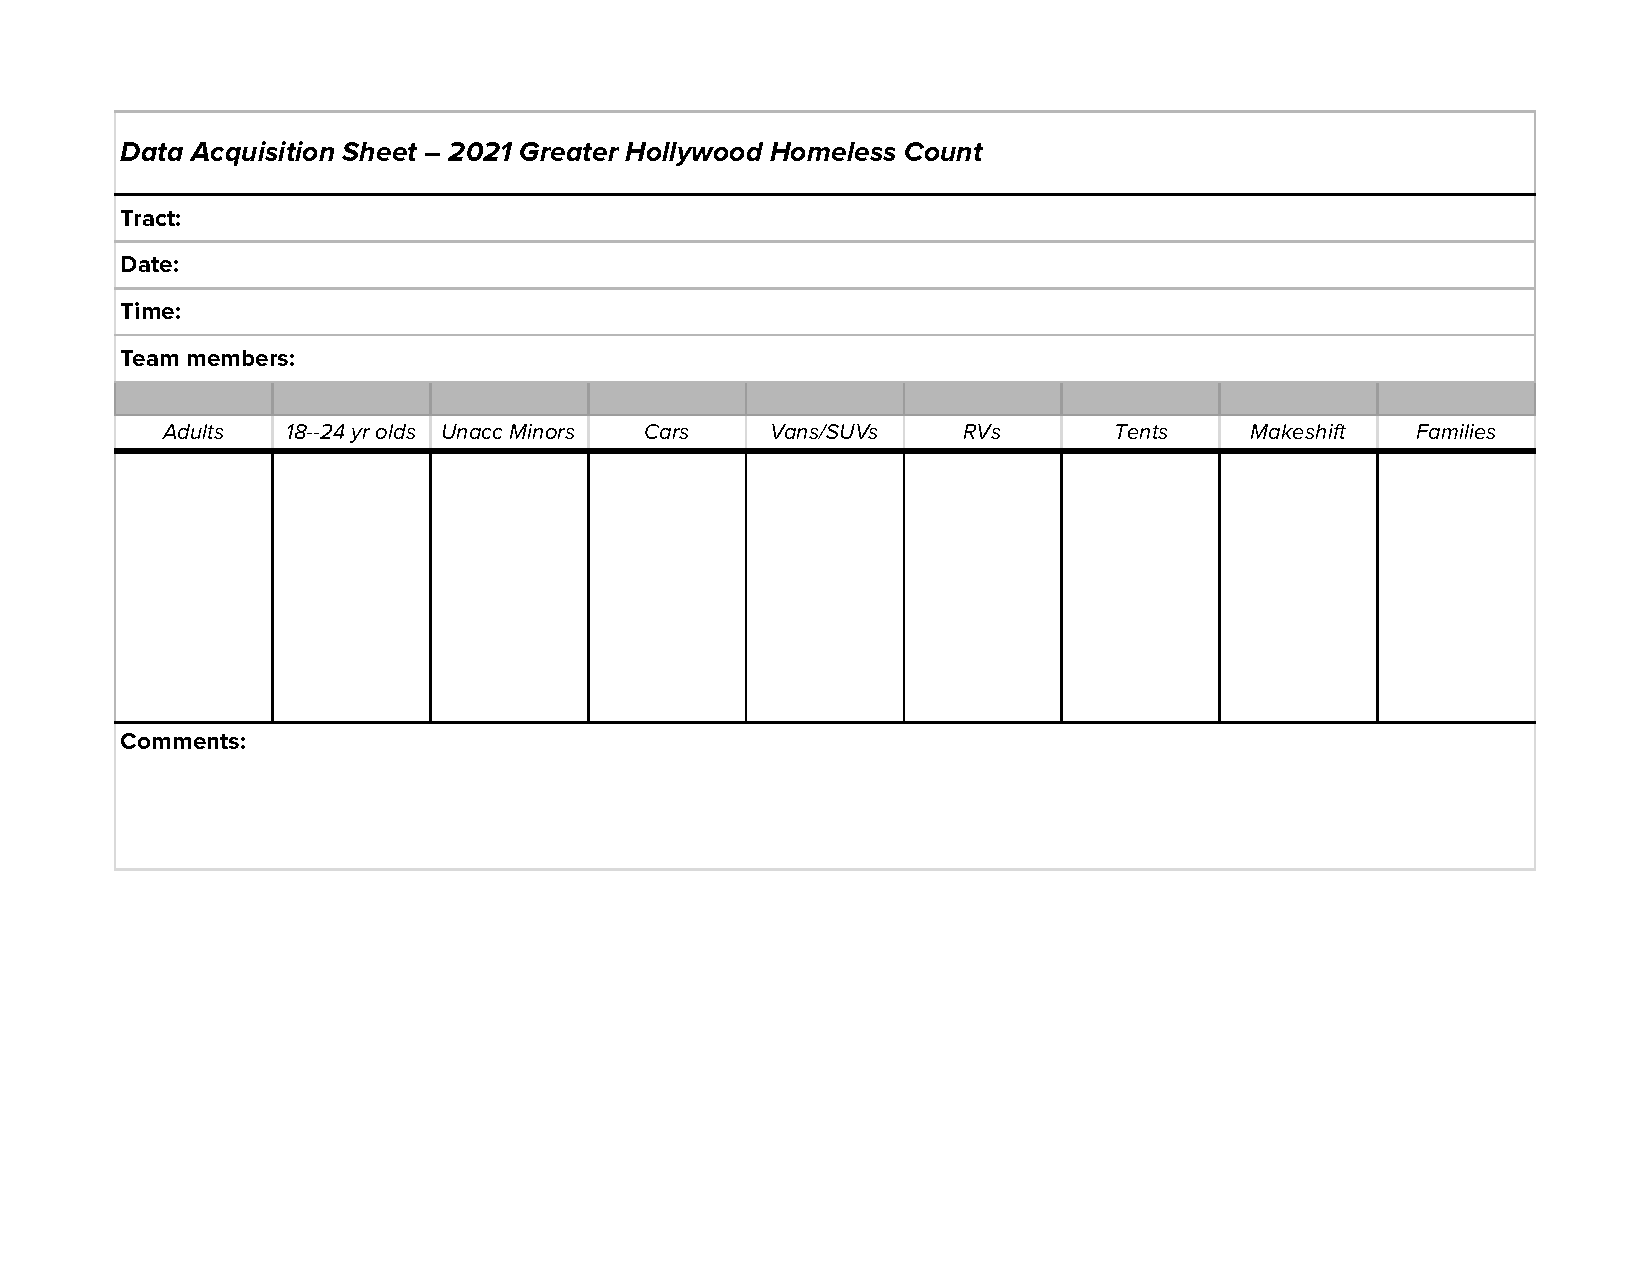
\includegraphics[width =\linewidth]{Hollywood2021CountDataSheet}
	\caption{Counter tally-sheet}
\end{figure*}

\begin{figure*}
	\centering
	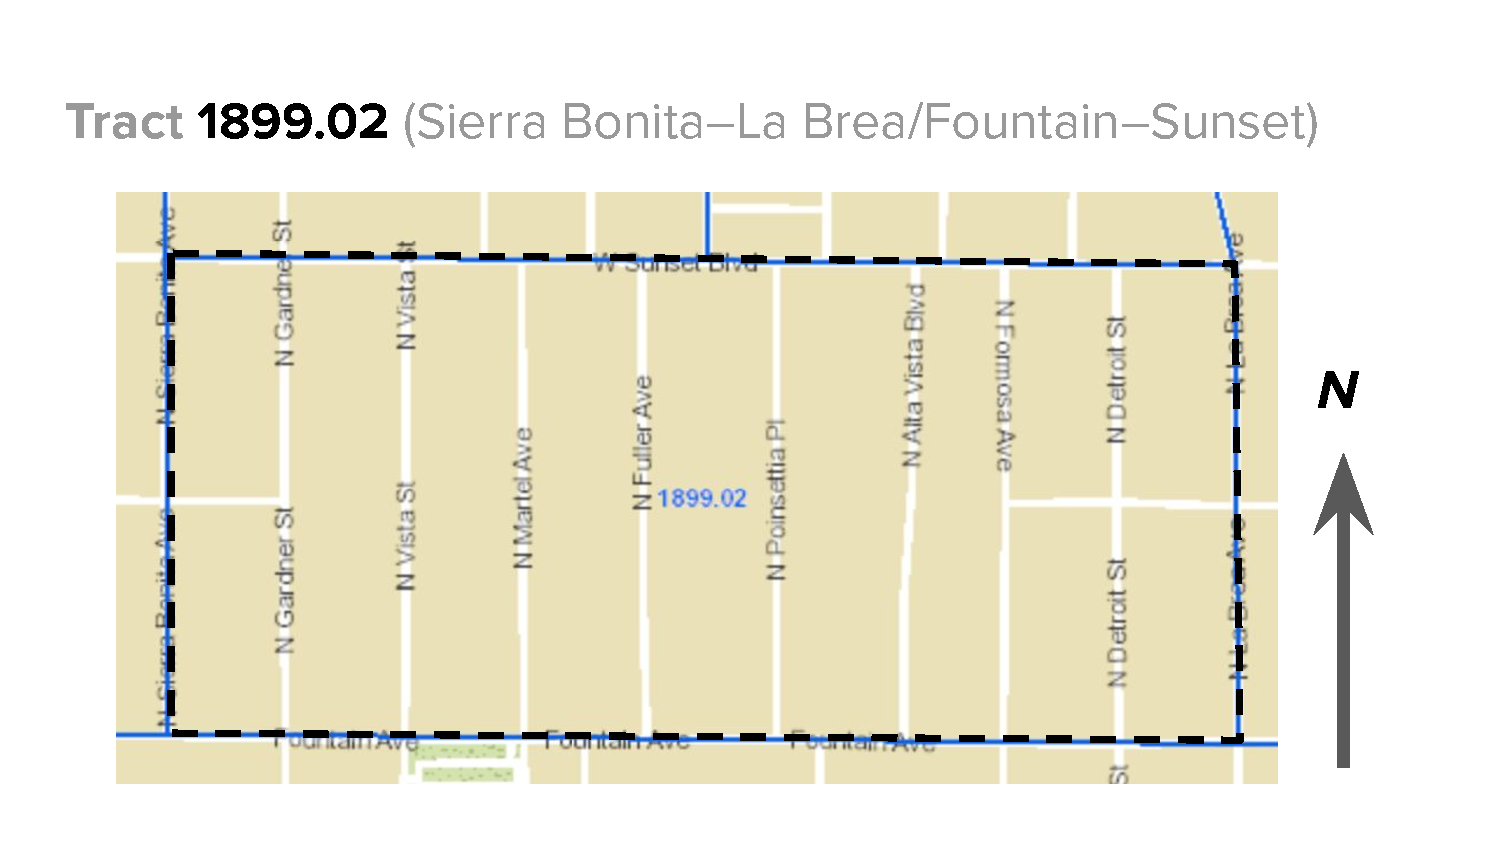
\includegraphics[width =\linewidth]{tractMap}
	\caption{Example Hollywood tract map.}
\end{figure*}

\begin{figure*}
	\centering
	\includegraphics[width =0.7\linewidth]{primerFront}
	\caption{Count primer {\bfr SCRUB EK'S NUMBER!}}
\end{figure*}

\section{Full Tract-level Results}

\begin{table*}[]
\caption{Census Tract-level Unsheltered Counts}
%\resizebox{\textwidth}{!}{%
\centering
\begin{tabular}{ccccccccccc}
\toprule
Tract & Community & Counter & $A$ & {\it TAY} & $C$ & $V$ & $R$ & $T$ & $M$ & {\bf Total} \\ \cmidrule{1-11}
1898.00 & Hollywood & V &  3.3 &  0.3 &  0.0 &  0.7 & 0 &  1.3 &  0.0 &   5.7 \\
1899.02 & Hollywood & V &  4.3 &  0.0 &  0.0 &  1.3 & 2 &  4.0 &  1.3 &  13.7 \\
1899.03 & Hollywood & V &  0.0 &  0.0 &  0.0 &  0.0 & 0 &  0.0 &  0.0 &   0.0 \\
1899.04 & Hollywood & V &  9.5 &  0.0 &  0.0 &  1.0 & 0 &  2.5 &  2.0 &  15.0 \\
1899.05 & Hollywood & V &  3.0 &  0.0 &  3.0 &  4.5 & 1 &  2.0 &  0.0 &  13.5 \\
1901.00 & Hollywood & V & 49.5 &  0.5 &  8.0 &  5.5 & 1 &  6.0 &  4.0 &  74.5 \\
1902.01 & Hollywood & V & 14.5 &  0.0 &  0.5 &  0.0 & 0 &  2.5 &  1.5 &  19.0 \\
1902.02 & Hollywood & V &  9.0 &  0.0 &  0.0 &  0.0 & 0 &  8.0 &  5.5 &  22.5 \\
1903.01 & Hollywood & P & 10.0 &  0.0 &  0.0 &  0.0 & 0 & 19.0 & 22.0 &  51.0 \\
1905.10 & Hollywood & P & 13.0 &  0.0 &  0.0 &  0.0 & 4 &  6.0 &  4.0 &  27.0 \\
1905.20 & E.~Hollywood & V &  2.0 &  0.5 &  0.5 &  1.0 & 0 &  4.0 &  1.0 &   9.0 \\
1907.00 & Hollywood & V & 38.5 &  0.0 &  2.0 &  0.0 & 0 & 38.5 &  7.0 &  86.0 \\
1908.01 & Hollywood & V & 18.5 &  0.0 &  0.5 &  0.0 & 0 & 19.5 &  9.0 &  47.5 \\
1908.02 & Hollywood & P & 22.0 &  0.0 &  0.0 &  1.0 & 5 & 13.0 & 13.0 &  54.0 \\
1909.01 & Hollywood & P & 15.0 &  0.0 &  0.0 &  0.0 & 0 & 17.0 &  9.0 &  41.0 \\
1909.02 & Hollywood & V &  2.7 &  0.3 &  0.7 &  1.7 & 0 &  0.0 &  0.0 &   5.3 \\
1910.00 & Hollywood & P & 34.0 &  0.0 &  1.0 &  0.0 & 5 & 60.0 & 23.0 & 123.0 \\
1911.10 & E.~Hollywood & V &  4.0 &  0.5 &  0.0 &  0.0 & 0 &  2.5 &  0.5 &   7.5 \\
1911.20 & E.~Hollywood & P & 14.0 &  0.0 &  0.0 &  0.0 & 0 & 24.0 & 10.0 &  48.0 \\
1912.01 & E.~Hollywood & V & 17.5 &  1.0 &  0.5 &  3.5 & 1 &  5.5 & 12.0 &  41.5 \\
1912.03 & E.~Hollywood & V &  5.0 &  0.0 &  2.0 &  8.0 & 0 &  0.0 &  2.5 &  17.5 \\
1912.04 & E.~Hollywood & V &  3.0 &  0.5 &  0.5 &  1.0 & 0 &  0.0 &  0.0 &   5.0 \\
1913.01 & E.~Hollywood & V &  8.0 &  0.0 &  0.5 &  7.5 & 0 &  5.0 &  1.0 &  22.5 \\
1913.02 & E.~Hollywood & V &  5.5 &  0.0 &  0.5 &  0.5 & 0 &  3.5 &  6.0 &  16.5 \\
1914.10 & E.~Hollywood & V &  7.5 &  0.0 &  1.0 &  0.5 & 0 &  1.0 &  5.5 &  15.5 \\
1914.20 & E.~Hollywood & V &  4.0 &  0.0 &  2.0 &  4.5 & 1 &  3.0 &  2.0 &  16.5 \\
1915.00 & E.~Hollywood & V & 10.0 &  0.0 &  0.0 &  4.5 & 2 &  2.5 &  2.5 &  22.0 \\
1916.10 & E.~Hollywood & P &  6.0 &  0.0 &  0.0 &  1.0 & 1 &  2.0 & 22.0 &  32.0 \\
1916.20 & E.~Hollywood & P &  0.0 &  2.0 &  0.0 &  0.0 & 0 &  4.0 &  6.0 &  12.0 \\
1917.10 & Hollywood & V &  6.5 &  0.0 &  2.0 &  4.5 & 1 &  1.0 &  0.5 &  15.5 \\
1917.20 & Hollywood & V &  2.3 &  0.0 &  0.3 &  1.3 & 6 &  0.0 &  4.3 &  14.7 \\
1918.10 & Hollywood & V &  3.5 &  0.0 &  1.0 &  1.5 & 1 & 10.0 &  0.0 &  17.5 \\
1918.20 & Hollywood & V &  2.5 &  1.0 &  0.0 &  2.5 & 2 &  1.5 &  2.0 &  11.5 \\
1919.01 & Hollywood & V & 16.0 &  0.0 &  2.0 &  1.5 & 5 & 13.0 &  7.5 &  45.0 \\
1925.10 & E.~Hollywood & V &  4.0 &  0.0 &  1.5 &  1.0 & 1 &  0.0 &  1.5 &   9.5 \\
1925.20 & E.~Hollywood & V &  1.0 &  0.0 &  1.0 &  6.0 & 1 &  0.0 &  0.0 &   9.0 \\
1926.10 & E.~Hollywood & V &  2.0 &  0.0 &  0.0 &  0.0 & 0 &  3.5 &  0.5 &   6.0 \\
1926.20 & E.~Hollywood & V &  1.0 &  0.0 &  0.0 &  0.0 & 0 & 11.0 &  0.5 &  12.5 \\
1927.00 & E.~Hollywood & P & 20.0 &  0.0 &  0.0 &  0.0 & 7 &  6.0 & 54.0 &  87.0 \\
\bottomrule
\end{tabular}
%}
\caption*{Raw counts from each tract. Coding as in Table \ref{tbl:tractStats}. Fractional counts
reflect averages over multiple counters.}
\label{tbl:allCount}
\end{table*}

\begin{table*}[]
\caption{Census Tract-level Unsheltered Population Inferences}
\resizebox{\linewidth}{!}{
\begin{tabular}{ccccccccccc}
\toprule
Tract & Community & Counter & $A$ & {\it TAY} & $C$ & $V$ & $R$ & $T$ & $M$ & {\bf Total}\\ \cmidrule{1-11}
1898.00 & H & V &  3.3 ( 1.7) &  0.0 ( 0.6) &  0.0 ( 2.2) &  0.0 ( 1.5) &  0.0 ( 2.8) &  1.9 ( 1.6) &  0.0 ( 7.0) &   6.9 (  8.4) \\
1899.02 & H & V &  4.3 ( 2.0) &  0.0 ( 0.7) &  0.0 ( 2.3) &  2.3 ( 2.2) &  3.8 ( 2.5) &  5.9 ( 2.9) &  2.2 ( 2.0) &  18.7 (  5.8) \\
1899.03 & H & V &  0.0 ( 5.2) &  0.0 ( 0.7) &  0.0 ( 2.2) &  0.0 ( 3.9) &  0.0 ( 2.8) &  0.0 ( 6.8) &  0.0 ( 7.1) &   0.0 ( 12.3) \\
1899.04 & H & V &  9.5 ( 3.6) &  0.0 ( 0.7) &  0.0 ( 2.3) &  0.0 ( 2.2) &  0.0 ( 2.7) &  3.7 ( 2.7) &  3.3 ( 3.0) &  18.3 (  7.0) \\
1899.05 & H & V &  3.0 ( 2.0) &  0.0 ( 0.7) &  4.4 ( 3.3) &  7.7 ( 5.4) &  0.0 ( 1.7) &  2.9 ( 2.5) &  0.0 ( 7.1) &  19.9 ( 10.3) \\
1901.00 & H & V & 49.5 ( 8.2) &  0.0 ( 0.8) & 11.8 ( 5.9) &  9.5 ( 6.1) &  0.0 ( 1.8) &  8.9 ( 4.3) &  6.6 ( 4.5) &  88.8 ( 13.5) \\
1902.01 & H & V & 14.5 ( 4.4) &  0.0 ( 0.7) &  0.0 ( 1.3) &  0.0 ( 3.9) &  0.0 ( 2.8) &  3.7 ( 2.8) &  0.0 ( 2.5) &  21.5 (  7.7) \\
1902.02 & H & V &  9.0 ( 3.5) &  0.0 ( 0.7) &  0.0 ( 2.2) &  0.0 ( 4.0) &  0.0 ( 2.8) & 11.8 ( 5.0) &  9.1 ( 5.3) &  30.2 (  9.9) \\
1903.01 & H & P & 10.0 ( 5.2) &  0.0 ( 0.7) &  0.0 ( 2.2) &  0.0 ( 3.9) &  0.0 ( 2.7) & 27.8 (11.0) & 36.5 (16.8) &  74.8 ( 21.3) \\
1905.10 & H & P & 12.9 ( 5.9) &  0.0 ( 0.7) &  0.0 ( 2.2) &  0.0 ( 4.0) &  5.7 ( 5.1) &  8.8 ( 6.0) &  6.5 ( 5.9) &  34.2 ( 12.4) \\
1905.20 & E & V &  2.0 ( 1.6) &  0.0 ( 0.8) &  0.0 ( 1.3) &  0.0 ( 2.2) &  0.0 ( 2.8) &  5.9 ( 3.6) &  0.0 ( 2.1) &  12.7 (  6.0) \\
1907.00 & H & V & 38.5 ( 7.2) &  0.0 ( 0.7) &  3.0 ( 2.6) &  0.0 ( 3.9) &  0.0 ( 2.8) & 56.7 (12.8) & 11.6 ( 6.3) & 110.1 ( 16.9) \\
1908.01 & H & V & 18.5 ( 4.9) &  0.0 ( 0.7) &  0.0 ( 1.3) &  0.0 ( 3.9) &  0.0 ( 2.8) & 28.6 ( 8.4) & 14.9 ( 7.4) &  63.2 ( 13.2) \\
1908.02 & H & P & 21.9 ( 7.7) &  0.0 ( 0.7) &  0.0 ( 2.2) &  0.0 ( 3.1) &  7.1 ( 5.8) & 19.0 ( 9.1) & 21.3 (11.8) &  71.7 ( 18.1) \\
1909.01 & H & P & 15.0 ( 6.3) &  0.0 ( 0.7) &  0.0 ( 2.3) &  0.0 ( 4.0) &  0.0 ( 2.8) & 24.9 (10.6) & 14.8 ( 9.4) &  55.3 ( 16.4) \\
1909.02 & H & V &  2.7 ( 1.5) &  0.0 ( 0.6) &  0.0 ( 1.2) &  2.9 ( 2.5) &  0.0 ( 2.7) &  0.0 ( 6.8) &  0.0 ( 7.2) &   6.9 ( 10.7) \\
1910.00 & H & P & 34.0 ( 9.6) &  0.0 ( 0.7) &  0.0 ( 2.6) &  0.0 ( 3.9) &  7.0 ( 5.7) & 88.1 (21.7) & 38.1 (17.4) & 169.7 ( 30.4) \\
1911.10 & E & V &  4.0 ( 2.3) &  0.0 ( 0.8) &  0.0 ( 2.2) &  0.0 ( 3.9) &  0.0 ( 2.7) &  3.6 ( 2.8) &  0.0 ( 1.4) &   9.0 (  6.7) \\
1911.20 & E & P & 13.9 ( 6.1) &  0.0 ( 0.7) &  0.0 ( 2.2) &  0.0 ( 3.9) &  0.0 ( 2.7) & 35.3 (12.8) & 16.4 (10.1) &  66.2 ( 18.2) \\
1912.01 & E & V & 17.5 ( 4.9) &  0.0 ( 1.1) &  0.0 ( 1.3) &  6.0 ( 4.6) &  0.0 ( 2.2) &  8.1 ( 4.2) & 19.9 ( 9.0) &  55.8 ( 12.4) \\
1912.03 & E & V &  5.0 ( 2.6) &  0.0 ( 0.7) &  3.0 ( 2.6) & 13.9 ( 7.8) &  0.0 ( 2.8) &  0.0 ( 6.8) &  4.2 ( 3.3) &  26.4 ( 11.9) \\
1912.04 & E & V &  3.0 ( 2.0) &  0.0 ( 0.8) &  0.0 ( 1.3) &  0.0 ( 2.2) &  0.0 ( 2.8) &  0.0 ( 6.8) &  0.0 ( 7.0) &   6.2 ( 10.7) \\
1913.01 & E & V &  8.0 ( 3.3) &  0.0 ( 0.7) &  0.0 ( 1.3) & 13.0 ( 7.5) &  0.0 ( 1.2) &  7.3 ( 3.9) &  0.0 ( 2.0) &  31.8 (  9.5) \\
1913.02 & E & V &  5.5 ( 2.7) &  0.0 ( 0.7) &  0.0 ( 1.3) &  0.0 ( 1.5) &  0.0 ( 1.2) &  5.1 ( 3.2) &  9.9 ( 5.6) &  23.1 (  7.5) \\
1914.10 & E & V &  7.5 ( 3.2) &  0.0 ( 0.7) &  0.0 ( 1.8) &  0.0 ( 1.6) &  0.0 ( 2.8) &  0.0 ( 1.7) &  9.0 ( 5.3) &  20.6 (  7.4) \\
1914.20 & E & V &  4.0 ( 2.3) &  0.0 ( 0.7) &  3.0 ( 2.7) &  7.7 ( 5.3) &  0.0 ( 1.8) &  4.4 ( 3.0) &  3.3 ( 3.0) &  24.1 (  8.0) \\
1915.00 & E & V & 10.0 ( 3.6) &  0.0 ( 0.7) &  0.0 ( 2.2) &  7.8 ( 5.3) &  3.5 ( 2.9) &  3.7 ( 2.7) &  4.1 ( 3.4) &  29.6 (  8.6) \\
1916.10 & E & P &  6.0 ( 4.0) &  0.0 ( 0.7) &  0.0 ( 2.3) &  0.0 ( 3.1) &  0.0 ( 2.4) &  0.0 ( 3.4) & 36.4 (16.9) &  48.7 ( 18.3) \\
1916.20 & E & P &  0.0 ( 5.2) &  0.0 ( 2.3) &  0.0 ( 2.3) &  0.0 ( 3.9) &  0.0 ( 2.8) &  5.8 ( 4.9) & 10.0 ( 7.5) &  17.9 ( 11.9) \\
1917.10 & H & V &  6.5 ( 3.0) &  0.0 ( 0.7) &  3.0 ( 2.6) &  7.8 ( 5.4) &  0.0 ( 1.7) &  0.0 ( 1.8) &  0.0 ( 1.4) &  21.3 (  7.4) \\
1917.20 & H & V &  2.3 ( 1.5) &  0.0 ( 0.7) &  0.0 ( 0.9) &  2.3 ( 2.1) &  9.0 ( 4.3) &  0.0 ( 6.8) &  7.1 ( 3.9) &  21.7 (  9.6) \\
1918.10 & H & V &  3.5 ( 2.2) &  0.0 ( 0.7) &  0.0 ( 1.8) &  0.0 ( 2.7) &  0.0 ( 2.2) & 14.6 ( 5.7) &  0.0 ( 6.9) &  24.6 ( 10.2) \\
1918.20 & H & V &  2.5 ( 1.8) &  0.0 ( 1.2) &  0.0 ( 2.3) &  4.3 ( 3.8) &  2.9 ( 2.6) &  2.2 ( 2.1) &  3.3 ( 3.0) &  16.4 (  6.7) \\
1919.01 & H & V & 16.0 ( 4.7) &  0.0 ( 0.7) &  2.9 ( 2.6) &  0.0 ( 2.7) &  7.1 ( 4.3) & 19.1 ( 6.6) & 12.4 ( 6.5) &  60.6 ( 11.9) \\
1925.10 & E & V &  4.0 ( 2.3) &  0.0 ( 0.7) &  0.0 ( 2.2) &  0.0 ( 2.2) &  0.0 ( 2.2) &  0.0 ( 6.7) &  0.0 ( 2.6) &  12.8 (  8.5) \\
1925.20 & E & V &  0.0 ( 1.6) &  0.0 ( 0.7) &  0.0 ( 2.5) & 10.5 ( 8.3) &  0.0 ( 2.4) &  0.0 ( 6.8) &  0.0 ( 7.1) &  14.8 ( 13.6) \\
1926.10 & E & V &  2.0 ( 1.6) &  0.0 ( 0.7) &  0.0 ( 2.3) &  0.0 ( 4.0) &  0.0 ( 2.8) &  5.1 ( 3.3) &  0.0 ( 1.4) &   8.0 (  6.7) \\
1926.20 & E & V &  0.0 ( 1.2) &  0.0 ( 0.7) &  0.0 ( 2.2) &  0.0 ( 4.0) &  0.0 ( 2.8) & 16.1 ( 6.1) &  0.0 ( 1.4) &  18.0 (  8.4) \\
1927.00 & E & P & 19.9 ( 7.4) &  0.0 ( 0.7) &  0.0 ( 2.3) &  0.0 ( 3.9) & 10.0 ( 7.0) &  8.8 ( 6.0) & 90.4 (33.2) & 129.4 ( 35.4) \\
\bottomrule
\end{tabular}
}
\caption*{Median and 90\% CI listed.}
\label{tbl:allPop}
\end{table*}

%\begin{table*}[]
%\caption{Tract 1898.00 Unsheltered Data}
%\resizebox{\linewidth}{!}{%
%\begin{tabular}{lcccccccccc}
%\toprule
% & Adult & TAY & Unacc Minor & Car & Van & RV & Tent & Makeshift & Family & {\bf Total} \\ \cmidrule{1-11}
%Counts & 3 & 0 & 0 & 0 & 0 & 0 & 1 & 1 & 0 & {\bf 5} \\
%Inhabitants & 3 (3) & 0 (1) & 0 (1) & 1 (2) & 1 (2) & 1 (2) & 2 (2) & 2 (2) & 0 (1) & {\bf 9 (6)} \\
%Category share & 0.31 (0.29) & 0.03 (0.10) & 0.03 (0.10) & 0.09 (0.18) & 0.10 (0.19) & 0.07 (0.16) & 0.16 (0.23) & 0.18 (0.24) & 0.03 (0.10) & - 
%\\ \bottomrule
%\end{tabular}
%}
%\caption*{Quantities in parentheses denote 95\% uncertainties (binomial in the case of the categories). Uncertainties larger than estimates imply that only upper limits can be stated confidently.}
%\label{tbl:}
%\end{table*}

\end{document}  